%COMPILATION: 
%clear; bibtex main.aux;pdflatex main.tex ;evince main.pdf &


%%%%%%%%%%%%%%%%%%%%%%%%%%%%%%%%%%%%%%%%%%%%%%%%%%%%%%%%%%%%%%%%%%%%%%%%%%%%%%%%%%%%%%%%%%%%%%%%%%%%%%%%%%%%%%%%%%%%%
%													INTERET METHODE													%
%%%%%%%%%%%%%%%%%%%%%%%%%%%%%%%%%%%%%%%%%%%%%%%%%%%%%%%%%%%%%%%%%%%%%%%%%%%%%%%%%%%%%%%%%%%%%%%%%%%%%%%%%%%%%%%%%%%%%
	
\chapter{Évaluation}
\label{sec:eval}
	L'objectif de cette partie est d'évaluer les bénéfices des connaissances à priori présentées dans le chapitre~\ref{chap:info_concept} (la région d'intérêt, le nombre de classes et les relations d'ordre). Elles sont déduites des représentations conceptuelles des connaissances topologiques et photométriques, dans le cas d'une analyse séquentielle.\\

Intuitivement, l'information topologique permet :

%	Dans le chapitre précédent (chap.~\ref{chap:info_concept}), nous avons mis en place les mécanismes du moteur d'inférence via le formalisme. Nous allons maintenant le mettre en application pour analyser des images numériques synthétiques puis médicales. Notre méthode illustrée figure~\ref{fig:method_schema}, repose sur plusieurs éléments, tout d'abord, de part les informations à priori topologiques ($G_T$), nous allons pouvoir appliquer des masques successifs à l'image (définis par le moteur d'inférence) pour :

\begin{itemize}
	\item[a)] d'éliminer les données polluantes : amélioration du pourcentage de données utiles ;
	\item[b)] réduire le volume des données à traiter : complexité et temps de calcul réduits.
\end{itemize}

%Ensuite, nous travaillerons sur l'histogramme de l'image restreint à la \gls{ROI} pour segmenter et identifier chaque classe puis ajuster le fenêtrage pour une classe particulière (la cible). Nous nous appuierons cette fois ci sur les informations photométriques à priori ($G_P$), toujours issues du moteur d'inférence. Ces informations nous permettent de :
L'information photométrique permet de :

\begin{itemize}
	\item[c)] connaître le nombre et l'ordre des classes à priori : paramétrage des algorithmes de segmentation ;
	\item[d)] initialiser les algorithmes de segmentation au plus proche des paramètres des classes attendues (moyenne, intervalle) : moins d'itérations lors de la segmentation.
\end{itemize}\vspace{1em}

	A partir de ces considérations intuitives, nous proposons d'effectuer un certain nombre de tests permettant d'illustrer quantitativement les bénéfices. Il s'agit d'un exercice délicat, comparativement aux procédures classiques d'évaluation de la performance de classification d'un algorithme de segmentation (e.g. mesure objective du taux de pixel correctement classés). En effet, dans notre contexte, cette évaluation ne dépend pas seulement de la nature des données, mais également de l'algorithme et de la procédure itérative d'analyse (la région d'intérêt varie à chaque itération). Par conséquent, ces mesures quantitatives reflètent probablement moins objectivement les bénéfices de notre approche que dans le cas d'un algorithme particulier. 

	Notre objectif prioritaire est de montrer des cas dans lesquels notre approche facilite le traitement, afin d'alimenter notre argumentaire, et ainsi, de discuter des affirmations précédentes, dans des cas concrets. Cette démarche sera poursuivie dans un cadre plus applicatif dans le chapitre suivant dédié à une application médicale.

	Après une courte présentation de l'algorithme utilisé pour réaliser cette évaluation, nous allons traiter chacun des points cités précédemment (a, b, c, d).
%Nous allons illustrer chacun de ces points par un exemple simple, même si certain paraissent logiques, afin de quantifier le bénéfice attendu pour notre application.

	%%%%%%%%%%%%%%%%%%%%%%%%%%%%%%%%%%%%%%%%%%%%%%%%%%%%%%%%%%%%%%%%%%%%%%%%%%%%%%%%%%%%%%%%%%%%%%%%%%%%%%%%%%%%%%%%%%%%%
	%													CHOIX OUTILS													%
	%%%%%%%%%%%%%%%%%%%%%%%%%%%%%%%%%%%%%%%%%%%%%%%%%%%%%%%%%%%%%%%%%%%%%%%%%%%%%%%%%%%%%%%%%%%%%%%%%%%%%%%%%%%%%%%%%%%%%
	\section{Algorithme considéré}
		%Suite à l'état de l'art sur les techniques de seuillage d'images (section~\ref{sec:state_of_the_art}), 
Nous avons choisi d'utiliser l'algorithme des \emph{K-Means} car il est largement répandu pour les raisons évoquées dans \citep[Ranjan]{Ranjan2010} ``\textit{the simplicity and computational speed of the K-means algorithm ... has made it a popular choice.}''. Cet algorithme nécessite néanmoins des paramètres d'initialisations pour calculer une segmentation pertinente \citep[Ranjan]{Ranjan2010} ``\textit{the algorithm needs initializing values which greatly influence its terminating optimal solution ... good initialization is crucial for finding globally optimal partitionings}''. 
		
		L'algorithme \emph{K-Means} est une méthode dont le but est de diviser $n$ observations $X$ en $k$ partitions (clusters) $V=\{V_1, V_2, …, V_k\}$ afin de minimiser la somme des carrés à la moyenne à l'intérieur de chaque partition (eq.~\ref{eq:kmean}).
		
		
		%vise à partitionner un nuage de données en plusieurs ensembles de points (clusters) en minimisant la somme des carrés à la moyenne à l'intérieur de chaque partition.


 \begin{equation}
 	\mathrm{arg\;min} \sum_{j=1}^k \sum_{n \in V_j} \left| X_n - \mu_j \right|^2
 	\label{eq:kmean}
 \end{equation}
  
% et d'autre part, parce qu'il détermine les bornes minimum et maximum d'un groupe de points : ce qui est précisément ce dont nous avons besoin pour fenêtrage.

	Les paramètres sont : le nombre de partitions $k$ et leurs moyennes respectives. Nous déterminerons $k$ par les connaissances contextuelles à priori. Pour l'initialisation des moyennes, on peut utiliser des moyens automatiques comme le tirage aléatoire de valeurs, l'algorithme \emph{K-Means++}\citep[Arthur2007]{Arthur2007} ou bien manuellement. %Nous préférerons, dans la mesure du possible, une initialisation manuelle à partir des connaissances à priori pour s'assurer d'un résultat optimal (et invariable).

	Le contexte d'utilisation de cet algorithme s'apparente à de la segmentation d'images par analyse d'histogramme (analyse de la distribution des intensités). Il s'agit d'une approche couramment considérée en traitement d'images, l'enjeu étant la détermination robuste des seuils discriminant les différentes régions d'une image (\citep[Coudray]{Coudray2010}, \citep[Bhattacharyya]{Bhattacharyya2011}, \citep[Cheng]{Cheng1998}, \citep[Cuevas]{Cuevas2010}). Le lecteur pourra également se référer à l'état de l'art de \citep[Zhang]{Zhang2008} sur ces méthodes.

	\vspace{1em}
		
		%{\bf Figure de la méthode supprimée : à voir si je l'adapte pour la présentation. JBF : A remplacer par un graphe liant les concepts (e.g. à gauche: GT, GP, inférence, roi, nb classes, ordre) et les bénéfices (e.g. à droite - correspond à a),b),c) et d)): titre possible "Méthode: information et bénéfices"}
	%%%%%%%%%%%%%%%%%%%%%%%%%%%%%%%%%%%%%%%%%%%%%%%%%%%
%	\begin{figure}[!ht]	%trim=l b r t  width=0.5\textwidth, 
%	  	\centering
%			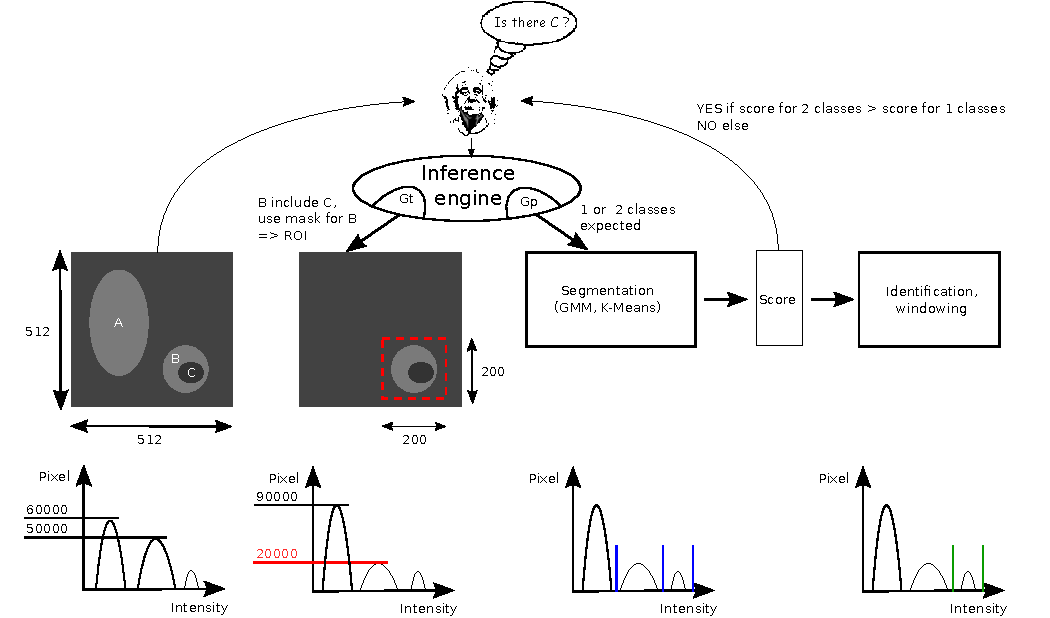
\includegraphics[trim= 0mm 0mm 0mm 0mm, clip, width=0.95\textwidth]{Evaluation/figure/method_schema.pdf}
%		\caption{Principe de la méthode:}
%		\label{fig:method_schema}
%	\end{figure}
	%%%%%%%%%%%%%%%%%%%%%%%%%%%%%%%%%%%%%%%%%%%%%%%%%%%
	
	
	%\section{Étude}
	%%%%%%%%%%%%%%%%%%%%%%%%%%%%%%%%%%%%%%%%%%%%%%%%%%%%%%%%%%%%%%%%%%%%%%%%%%%%%%%%%%%%%%%%%%%%%%%%%%%%%%%%%%%%%%%%%%%%%
	%												DONNEES POLLUANTES													%
	%%%%%%%%%%%%%%%%%%%%%%%%%%%%%%%%%%%%%%%%%%%%%%%%%%%%%%%%%%%%%%%%%%%%%%%%%%%%%%%%%%%%%%%%%%%%%%%%%%%%%%%%%%%%%%%%%%%%%

		\section{Élimination des données polluantes}
		\label{sec:data_reduction}
			\subsection*{Efficacité de segmentation}
	Ici nous allons illustrer l'atout des masques pour l'élimination des données polluantes de l'image. Ces données polluantes sont souvent caractérisées par des régions de l'image situées en dehors de la ROI (topologiquement) mais avec des intensités proche de celles se trouvant au sein de la ROI. Ces intensités sont donc confondues dans l'histogramme de l'image et biaisent la segmentation. En comparant les deux histogrammes, on voit clairement que les intensités de la région C se mélangent à celles des régions B et D (fig.~\ref{fig:me_1_hist_1} et ~\ref{fig:me_1_hist_2}).

	%%%%%%%%%%%%%%%%%%%%%%%%%%%%%%%%%%%%%%%%%%%%%%%%%%%
	\begin{figure}[!ht]	%trim=l b r t  width=0.5\textwidth, 
	  \centering
			\subfloat[Image (250x250)]{\label{fig:me_1_img_1}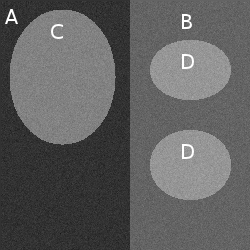
\includegraphics[trim= 0mm 0mm 0mm 0mm, clip, height=0.21\textwidth]{Evaluation/figure/me_1_0_img_1.png}}	\hspace{2em}
			\subfloat[Binarisation]{\label{fig:me_1_0_bin_1}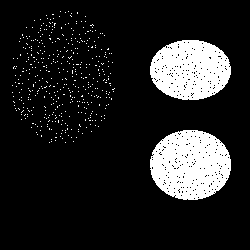
\includegraphics[trim= 0mm 0mm 0mm 0mm, clip, height=0.21\textwidth]{Evaluation/figure/me_1_0_bin_1.png}}	\hspace{2em}
			\subfloat[Histogramme image initiale]{\label{fig:me_1_hist_1}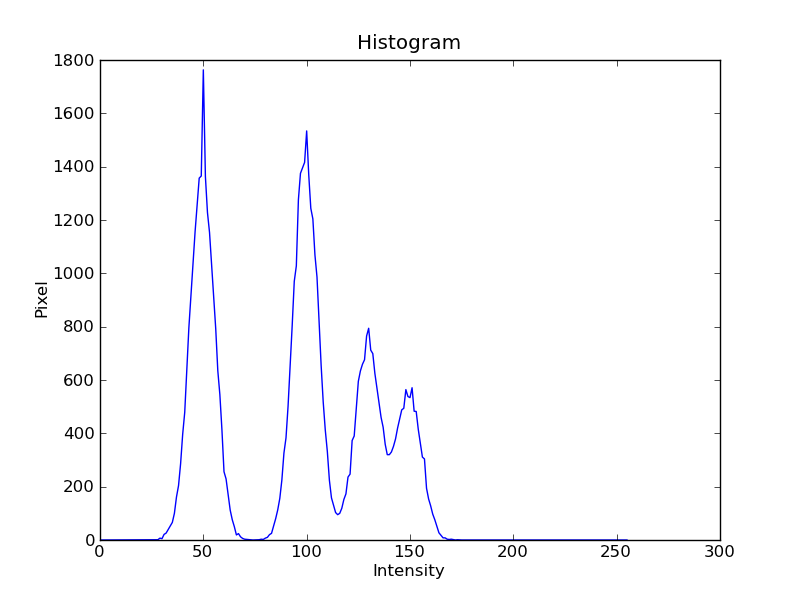
\includegraphics[trim= 5mm 5mm 5mm 5mm, clip, width=0.3\textwidth]{Evaluation/figure/me_1_0_hist_1.png}} \\
			\subfloat[Image masquée]{\label{fig:me_1_img_2}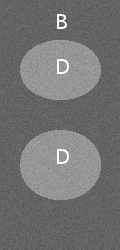
\includegraphics[trim= -25mm 0mm -25mm 0mm, clip, height=0.21\textwidth]{Evaluation/figure/me_1_0_img_2.png}}	\hspace{2em}
			\subfloat[Binarisation]{\label{fig:me_1_0_bin_2}
\includegraphics[trim= -25mm 0mm -25mm 0mm, clip, height=0.21\textwidth]{Evaluation/figure/me_1_0_bin_2.png}}	\hspace{2em}
			\subfloat[Histogramme image masquée]{\label{fig:me_1_hist_2}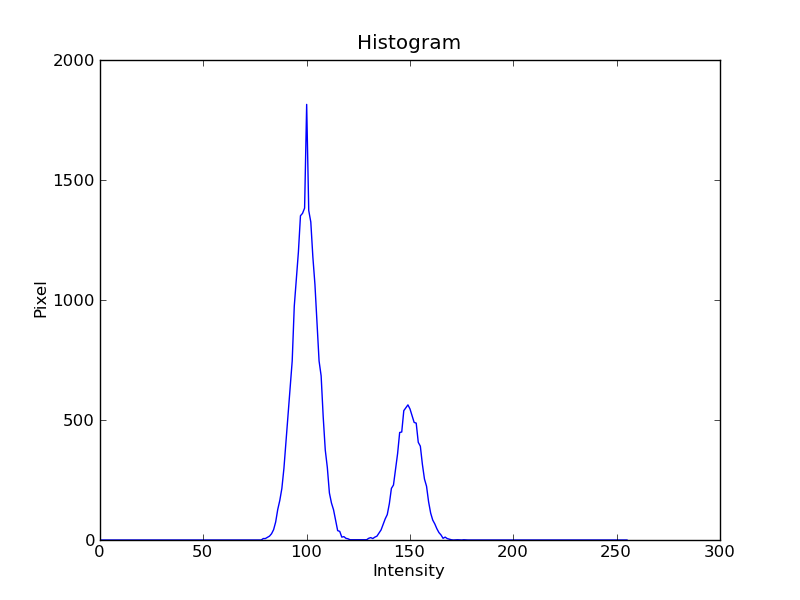
\includegraphics[trim= 5mm 5mm 5mm 5mm, clip, width=0.3\textwidth]{Evaluation/figure/me_1_0_hist_2.png}}
		  \caption{Images et histogrammes associés}
	\end{figure}
	%%%%%%%%%%%%%%%%%%%%%%%%%%%%%%%%%%%%%%%%%%%%%%%%%%%


	Afin de discuter de cet aspect, nous allons considérer le cas de la segmentation de la région D, en considérant que B ait été segmenté ou non:
\begin{itemize}
\item
Cas B segmenté : la segmentation de D se fait au sein de la région B (fig.~\ref{fig:me_1_img_2}) conduisant à un histogramme comprenant des lobes bien distincts (fig.~\ref{fig:me_1_hist_2}). L'application de \emph{K-Means} initialisé avec \emph{K-means++} permet une segmentation quasiment sans erreur de D (fig.~\ref{fig:me_1_0_bin_2}). Ce résultat aurait pu être vérifié avec un autre algorithme de segmentation. Le nombre de faux positifs \footnote{Faux positifs (FP) : points considérés comme appartenant à la région cible (e.g. D) à tort.} et faux négatifs \footnote{Faux négatifs (FN) : points considérés comme n'appartenant pas à la région cible (e.g. D) à tort.} sont très faibles, respectivement 2 et 0.
\item
Cas B non segmenté : la segmentation de D se fait en considérant toute l'image (fig.~\ref{fig:me_1_img_1}). L'application de \emph{K-Means} dans les mêmes conditions que précédemment conduit à un seuil erroné (i.e. le seuil inférieur sera trop élevé, correspondant à la vallée entre les lobes C et D sur l'histogramme fig.~\ref{fig:me_1_hist_1} et non au minimum réel de D). Davantage de points sont classés comme n'appartenant pas à D : le taux de faux négatifs augmente grandement (761 pixels). Inversement, un certain nombre de point de C sont, par erreur, associés à la région D : le taux de faux positifs augmente également (352 pixels).
\end{itemize}\vspace{1em}

Il est à noter qu'afin de pouvoir comparer les deux approches, il semble plus pertinent de focaliser la comparaison sur les points de D qui ne sont pas associés à D après segmentation alors qu'ils devraient l'être (faux négatifs): on ignore alors les performances de classification en dehors de D, ceci dépendant de la ROI au sein de laquelle les traitements sont effectués (très variable en fonction des structures externes à D). Par conséquent, le seul critère significatif à notre sens est celui faisant intervenir les vrais positifs et les faux négatifs : la sensibilité \footnote{Sensibilité: proportion de points positifs qui ont été classés positifs : VP / (VP + FN), VP désignant les vrai positifs (points considérés comme appartenant à la région cible à raison).}. La spécificité \footnote{Spécificité: Proportion de points négatifs qui ont été classés négatifs : VN / (VN + FP), VN désignant les vrais négatifs (points considérés comme n'appartenant pas à la région cible à raison).} ne faisant intervenir que les vrai négatifs et les faux positifs.

\begin{center}
	\begin{minipage}[b]{0.5\linewidth}
		\centering
			\begin{tabular}{|l|cccc|}
			\hline
				\textbf{Région D}& \multicolumn{2}{|c|}{\textbf{C non masqué}} 	& \multicolumn{2}{|c|}{\textbf{C masqué}} \\
				\hline
							& Vrai	& Faux 		& Vrai	& Faux 		\\
				\hline
					Positif	& 8018 	&  352 		& 8368 	& 2 	 	\\
				 	Négatif	& 53369 &  761		& 21630	& 0		\\
			\hline
				Sensibilité	& \multicolumn{2}{|c|}{91.33\%} 	& \multicolumn{2}{|c|}{100\%} \\
				Spécificité	& \multicolumn{2}{|c|}{99.35\%} 	& \multicolumn{2}{|c|}{99.99\%} \\
				\hline
			\end{tabular}
			\captionof{table}{Classement des pixels}
			\label{tab:mask_effect_D}
	\end{minipage}
\end{center}

% MASQUE, THRESHOLD AND BINARISATION OF MEDICAL IMAGE TO DO PROPERLY

%	 Prenons cette fois ci comme exemple une image médicale, constituée du foie, de tumeurs du foie et de la rate, dans laquelle on recherche à segmenter les tumeurs du foie. On sait qu'une tumeur du foie n'est pas inclus dans la rate (topologiquement) : on peut donc masquer la rate sans perdre d'information sur les tumeurs. Mesurons le gain de sensibilité et la spécificité lors de la segmentation :


	%%%%%%%%%%%%%%%%%%%%%%%%%%%%%%%%%%%%%%%%%%%%%%%%%%%
%	\begin{figure}[!ht]	%trim=l b r t  width=0.5\textwidth, 
%	  \centering
%			\subfloat[Foie + tumeurs + rate]{\label{fig:apl_0_0_img1}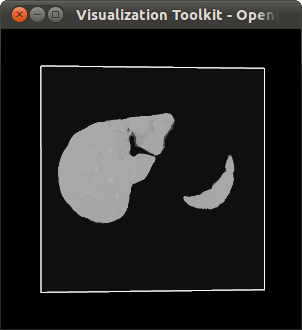
\includegraphics[trim= 15mm 30mm 20mm 30mm, clip, width=0.2\textwidth]{Evaluation/figure/apl_0_0_img1.png}}	\hspace{1em}
%			\subfloat[Segmentation]{\label{fig:apl_0_0_bw1}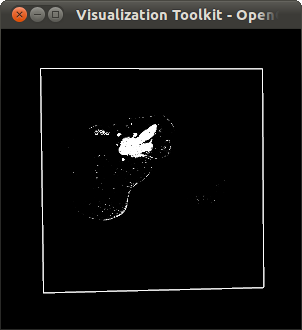
\includegraphics[trim= 15mm 30mm 20mm 30mm, clip, width=0.2\textwidth]{Evaluation/figure/apl_0_0_bw1.png}}	\hspace{1em}
%			\subfloat[Foie + tumeurs]{\label{fig:apl_0_0_img2}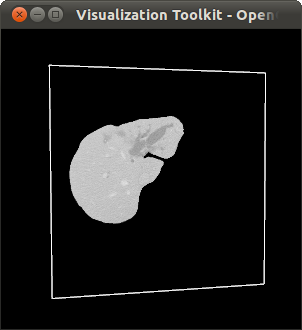
\includegraphics[trim= 20mm 30mm 20mm 34mm, clip, width=0.2\textwidth]{Evaluation/figure/apl_0_0_img2.png}}	\hspace{1em}
%			\subfloat[Segmentation]{\label{fig:apl_0_0_bw2}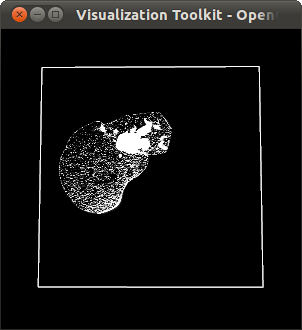
\includegraphics[trim= 15mm 30mm 20mm 30mm, clip, width=0.2\textwidth]{Evaluation/figure/apl_0_0_bw2.png}}
%		  \caption{Images et histogrammes associés}
%		  \label{fig:apl_1_1}
%	\end{figure}
	%%%%%%%%%%%%%%%%%%%%%%%%%%%%%%%%%%%%%%%%%%%%%%%%%%%


%\begin{center}
%	\begin{tabular}{|l|cccc|}
%		\hline
%		\textbf{Région tumeur}& \multicolumn{2}{|c|}{\textbf{Rate non masquée}} 	& \multicolumn{2}{|c|}{\textbf{Rate masquée}} \\
%		\hline
%					& Vrai		& Faux 					& Vrai		& Faux 	\\
%		\hline
%			Positif	& 1004 		& 13248 				& 1773 		& 13079 	 \\
%		 	Négatif	& 52308848 	& 105700				& 52308919 	& 105629 \\
%		\hline
%		Sensibilité	& \multicolumn{2}{|c|}{0.94\%}	& \multicolumn{2}{|c|}{1.65\%} \\
%		Spécificité	& \multicolumn{2}{|c|}{99.97\%} & \multicolumn{2}{|c|}{99.97\%} \\
%		\hline
%	\end{tabular}
%	\captionof{table}{Effet du masquage de la rate}
%	\label{tab:apl_1_0_mask_effect_B}
%\end{center}

	 

%%%%%%%%%%%%%%%%%%%%%%%%%%%%%%%%%%%%%%%%%%%%%%%%%%%%%%%%%%%%%%%%%%%%%%%%%%%%%%%%%%%%%%%%%%%%%%%%%%%%%%%%%%%%%%%%%%%%%
%												TEMPS DE CONVERGENCE												%
%%%%%%%%%%%%%%%%%%%%%%%%%%%%%%%%%%%%%%%%%%%%%%%%%%%%%%%%%%%%%%%%%%%%%%%%%%%%%%%%%%%%%%%%%%%%%%%%%%%%%%%%%%%%%%%%%%%%%
\subsection*{Temps de calcul}
		Illustrons le fait que, pour un même volume de données à traiter, que le nombre moyen d'itération des algorithmes de segmentation tel que \emph{K-Means} dépend du nombre de classes de l'image. Comparons les trois images synthétiques ci-dessous (fig.~\ref{fig:me_1_3_img_0}, ~\ref{fig:me_1_3_img_1} et ~\ref{fig:me_1_3_img_2}) et calculons le nombre d'itérations moyen, pour 50 essais, que met l'algorithme pour converger vers leurs nombre de classes respectifs.
		
	%%%%%%%%%%%%%%%%%%%%%%%%%%%%%%%%%%%%%%%%%%%%%%%%%%%
	\begin{figure}[!ht]	%trim=l b r t  width=0.5\textwidth, 
	  \centering
			\subfloat[5 classes]{\label{fig:me_1_3_img_0}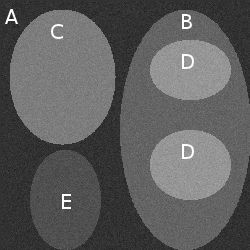
\includegraphics[trim= 0mm 0mm 0mm 0mm, clip, width=0.162\textwidth]{Evaluation/figure/me_1_3_img_0.png}}	\hspace{2em}
			\subfloat[4 classes]{\label{fig:me_1_3_img_1}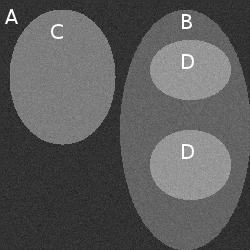
\includegraphics[trim= 0mm 0mm 0mm 0mm, clip, width=0.162\textwidth]{Evaluation/figure/me_1_3_img_1.png}}	\hspace{2em}
			\subfloat[3 classes]{\label{fig:me_1_3_img_2}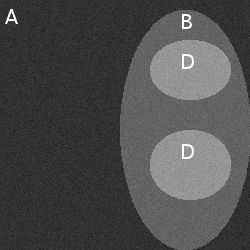
\includegraphics[trim= 0mm 0mm 0mm 0mm, clip, width=0.162\textwidth]{Evaluation/figure/me_1_3_img_2.png}}	\hspace{2em}
			%\subfloat[Binarisation]{\label{fig:apl_0_0_bw2}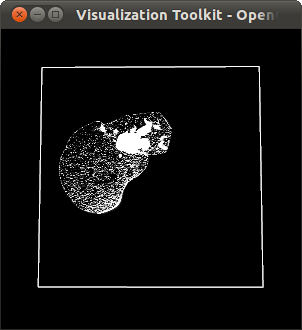
\includegraphics[trim= 15mm 30mm 20mm 30mm, clip, width=0.2\textwidth]{Evaluation/figure/apl_0_0_bw2.png}}
		  \caption{Images synthétiques ayant un nombre de classe différent.}
		  \label{fig:apl_1_0}
	\end{figure}
	%%%%%%%%%%%%%%%%%%%%%%%%%%%%%%%%%%%%%%%%%%%%%%%%%%%
	
	Il apparaît que, indépendamment du volume de données, le nombre de classes de l'image influence le temps de traitement (voir tableau~\ref{tab:convergence_time}). Ceci souligne donc un second intérêt d'éliminer les données polluantes car elles peuvent augmenter le nombre de classes et donc ralentir l'analyse. Ceci contribue également à montrer l'intérêt de réduire les analyses à une région d'intérêt, en ignorant les données polluantes, et ce même si elles ne diminuent pas la performance de la segmentation (e.g. données polluantes bien distinctes, en terme de lobe sur l'histogramme, des  lobes d'intérêt). Il est à noter que cette observation dépend fortement de la nature de l'algorithme de segmentation choisi car certains ne dépendent pas du nombre de classes.

\begin{center}
		\begin{tabular}{c|c|c|c|}

		\cline{2-4}
					& \textbf{Image 5 classes}		& \textbf{Image 4 classes} 	& \textbf{Image 3 classes} 	\\
		\cline{1-4}
	 	\multicolumn{1}{|c|}{\textbf{Nombre d'itérations}} & 6.34	 		& 3.52			& 1.2			\\
	 	 \cline{1-4}
%		\multicolumn{1}{|c|}{4 classes}			& 5.28 			& 3.52 			& 3.08			\\
%		\cline{1-5}
	\end{tabular}
	\captionof{table}{Nombre d'itérations moyen pour 50 essais par image}
	\label{tab:convergence_time}
\end{center}


%		La réduction du nombre de classes (e.g. masquage) permet bien de diminuer le nombre d'itérations et donc le temps de calcul des algorithmes de segmentation.



%%%%%%%%%%%%%%%%%%%%%%%%%%%%%%%%%%%%%%%%%%%%%%%%%%%%%%%%%%%%%%%%%%%%%%%%%%%%%%%%%%%%%%%%%%%%%%%%%%%%%%%%%%%%%%%%%%%%%
%													NOMBRE DE DONNÉES												%
%%%%%%%%%%%%%%%%%%%%%%%%%%%%%%%%%%%%%%%%%%%%%%%%%%%%%%%%%%%%%%%%%%%%%%%%%%%%%%%%%%%%%%%%%%%%%%%%%%%%%%%%%%%%%%%%%%%%%
		\section{Réduction de la quantité de données à traiter}
		Le temps de calcul est directement lié au nombre de données à traiter, quantifions ce gain à partir du tableau (tab.~\ref{tab:mask_effect_D}, région D). L'image (fig.~\ref{fig:me_1_img_1}) contient 250x250 pixels, le temps moyen de convergence avec \emph{K-Means} (10 itérations) est de 1,2 secondes sans masque et 0,8 secondes avec masque (fig.~\ref{fig:me_1_img_1} de 130x250 pixels). On considérera un gain d'environ de \textbf{30\%}.
		
		Les masques sont d'autant plus bénéfiques pour les images médicales puisque quelles contiennent beaucoup plus de données (de l'ordre de 512x512x$N$ pixels sans masque). Prenons comme exemple une image, constituée du foie, de tumeurs et de la rate, dans laquelle on recherche les tumeurs du foie (en rouge sur l'histogramme~\ref{fig:apl_1}), on sait qu'une tumeur du foie n'est pas, topologiquement, dans la rate (en vert sur l'histogramme~\ref{fig:apl_1_ltl}), on peut donc la masquer (voir l'histogramme~\ref{fig:apl_1_lt}). Les temps de calcul moyens pour trois (foie + tumeur + rate) puis deux (foie + tumeur) classes avec \emph{K-Means} (10 itérations) sont respectivement de 3,2 et 2,3 secondes. Soit un gain de \textbf{28\%}. Ces mesures ont été réalisées avec un processeur Intel Core 2 Duo à 2.66Ghz.



	%%%%%%%%%%%%%%%%%%%%%%%%%%%%%%%%%%%%%%%%%%%%%%%%%%%
	\begin{figure}[!ht]	%trim=l b r t  width=0.5\textwidth, 
	  \centering
			\subfloat[Image simplifiée]{\label{fig:ap_1_0_img}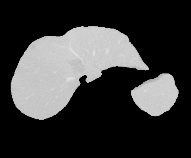
\includegraphics[trim= 0mm 0mm 0mm 0mm, clip, width=0.25\textwidth]{Evaluation/figure/ap_1_0_img.png}}
			\subfloat[Histogrammes global]{\label{fig:apl_1_ltl}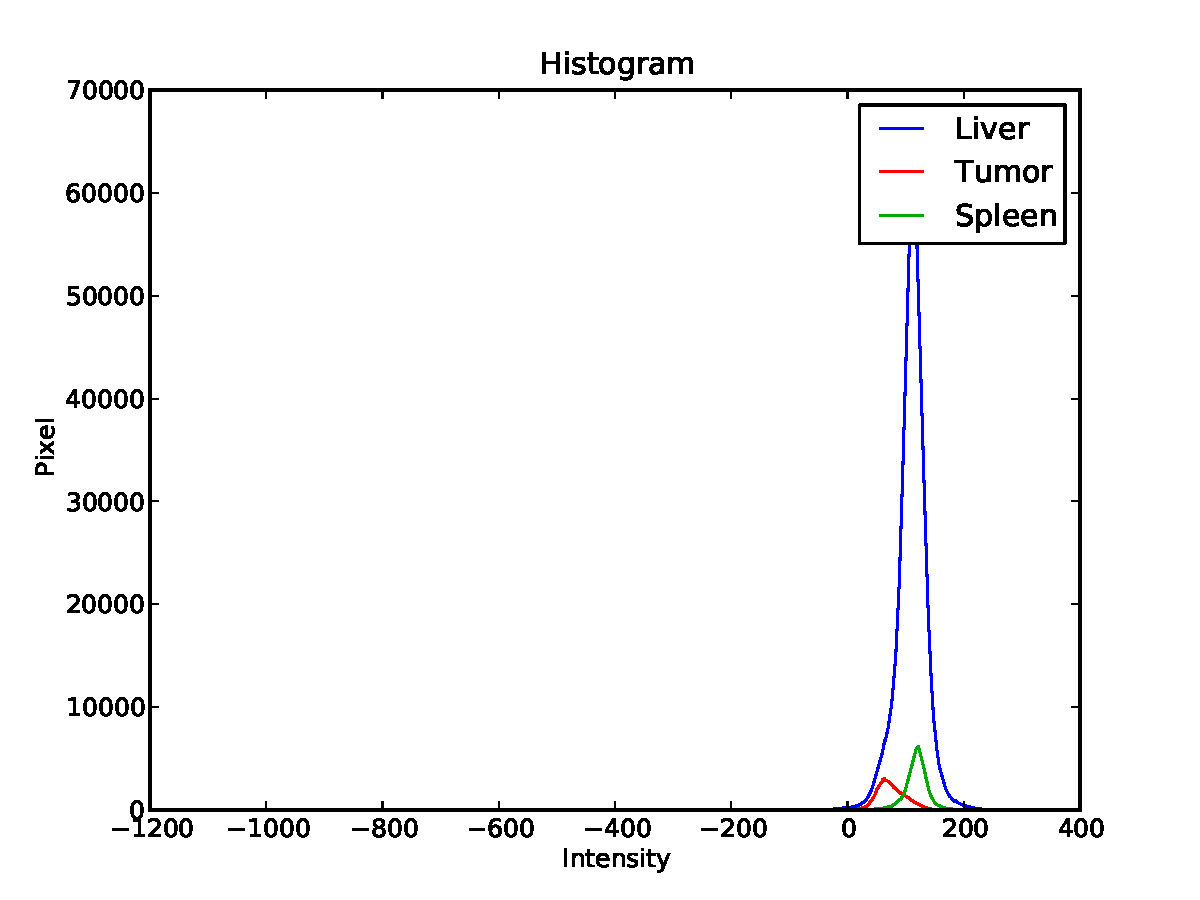
\includegraphics[trim= 5mm 5mm 5mm 5mm, clip, width=0.3\textwidth]{Evaluation/figure/apl_1_ltl.pdf}}
			\subfloat[Histogramme après masquage]{\label{fig:apl_1_lt}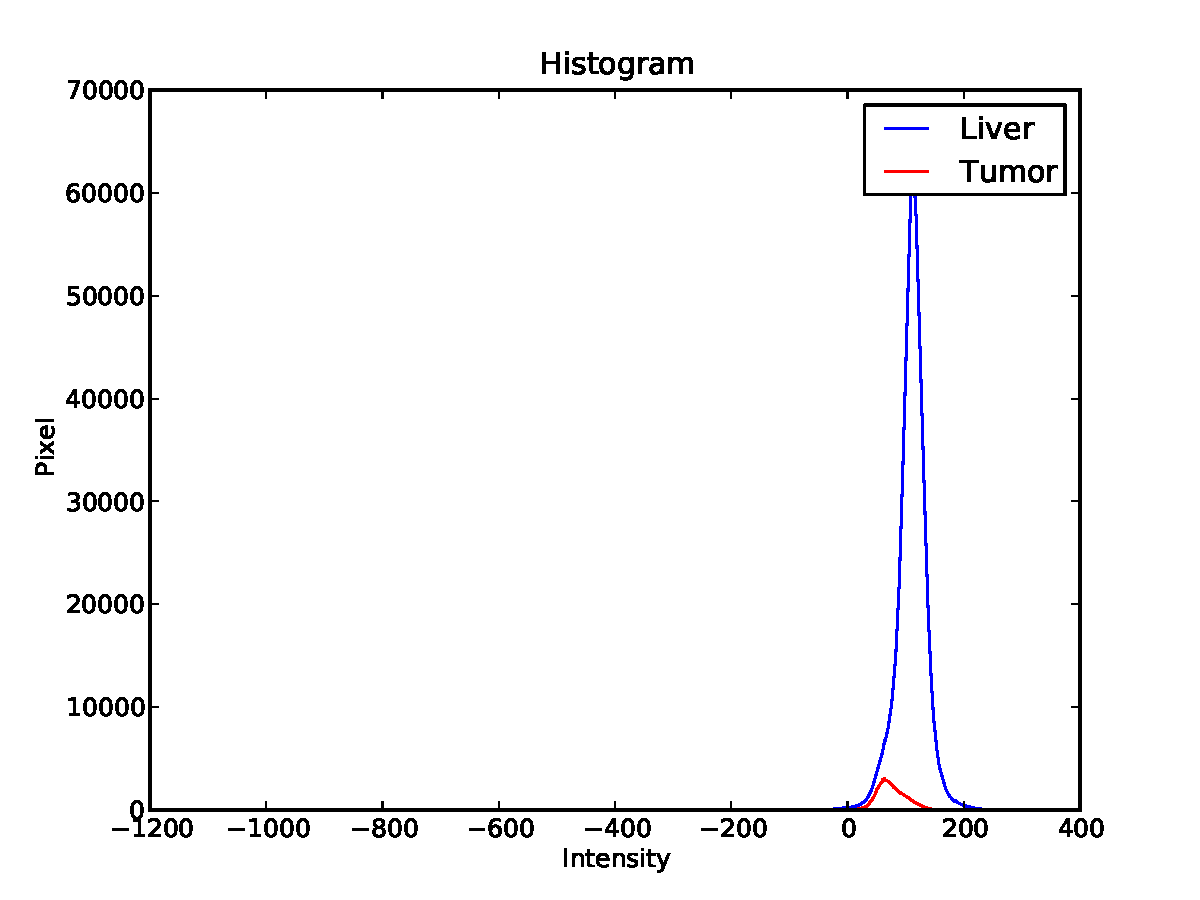
\includegraphics[trim= 5mm 5mm 5mm 5mm, clip, width=0.3\textwidth]{Evaluation/figure/apl_1_lt.pdf}}
		  \caption{Images et histogrammes associés}
		  \label{fig:apl_1}
	\end{figure}
	%%%%%%%%%%%%%%%%%%%%%%%%%%%%%%%%%%%%%%%%%%%%%%%%%%%

%%%%%%%%%%%%%%%%%%%%%%%%%%%%%%%%%%%%%%%%%%%%%%%%%%%%%%%%%%%%%%%%%%%%%%%%%%%%%%%%%%%%%%%%%%%%%%%%%%%%%%%%%%%%%%%%%%%%%
%												NOMBRE DE STRUCTURES												%
%%%%%%%%%%%%%%%%%%%%%%%%%%%%%%%%%%%%%%%%%%%%%%%%%%%%%%%%%%%%%%%%%%%%%%%%%%%%%%%%%%%%%%%%%%%%%%%%%%%%%%%%%%%%%%%%%%%%%
		\section{Connaissance du nombre de classe à priori}
		\label{subsec:nb_class}
	La connaissance du nombre à priori de classe dans l'image est un paramètre essentiel à certain algorithmes de segmentation comme \emph{K-Means} puisque c'est le nombre de classe qu'ils créent. Comme récemment souligné \citep[Ranjan]{Ranjan2010}, ceci est un point critique encore non résolu. Pour illustrer et discuter du bénéfice de la connaissance à priori du nombre de classes, nous allons considérer la méthode proposée par \citep[Ray]{Ray1999}. Il s'agit d'un choix arbitraire, sachant que d'autres méthodes auraient pu être utilisées (ceci pourrait faire l'objet d'une étude complémentaire). Cet algorithme d'estimation du nombre de classes est basé sur un critère de validité faisant intervenir le rapport entre les variances des classes et la distance minimum entre les classes obtenues par \emph{K-Means}. Cette mesure est réalisée pour un certain nombre de classes. Le nombre de classes optimal correspond au critère de validité minimum entre le premier maximum et la dernière valeur (correspondant au nombre maximum de classes). Une limitation est que cette méthode ne peut s'appliquer qu'à des données contenant au moins 4 classes.

En considérant cette approche automatique, nous allons discuter ci-après de l'intérêt de la connaissance à priori entre d'efficacité et de temps de calcul.


	\subsection*{Efficacité : les limites d'une détermination automatique}
Considérons une image synthétique à 8 classes (fig.~\ref{fig:me_3_3in1_1}), le critère proposé dans \citep[Ray]{Ray1999} permet d'automatiquement déterminer le nombre de classes, sans requérir de connaissance à priori supplémentaire : la courbe passe par un minimum à 8 correspondants au nombre de classes de l'image. On obtient donc une estimation correcte du nombre de classes.


Néanmoins, comme illustré par la figure~\ref{fig:me_3_3in1}, lorsque les classes apparaissent moins distinctes (voir ``data set'' fig.~\ref{fig:me_3_3in1}), on constate que l'estimation automatique échoue (la courbe indique une minimum pour 4 classes au lieu de 8), tandis que la connaissance à priori permet d'obtenir un résultat plus juste (voir la coloration des points dans la partie inférieure de ~\ref{fig:me_3_3in1}). Ceci peut être vu comme un résultat assez intuitif, c'est pourquoi il est rapporté afin d'illustrer uniquement le fait qu'il peut être plus efficace de disposer de connaissance a priori que de disposer d'un algorithme non supervisé qui viendrait compenser l'absence de connaissance a priori.
	

%		%%%%%%%%%%%%%%%%%%%%%%%%%%%%%%%%%%%%%%%%%%%%%%%%%%%
	\begin{figure}[!ht]	%trim=l b r t  width=0.5\textwidth, 
	  	\centering
	  		\subfloat[Classes distinctes]{\label{fig:me_3_3in1_1}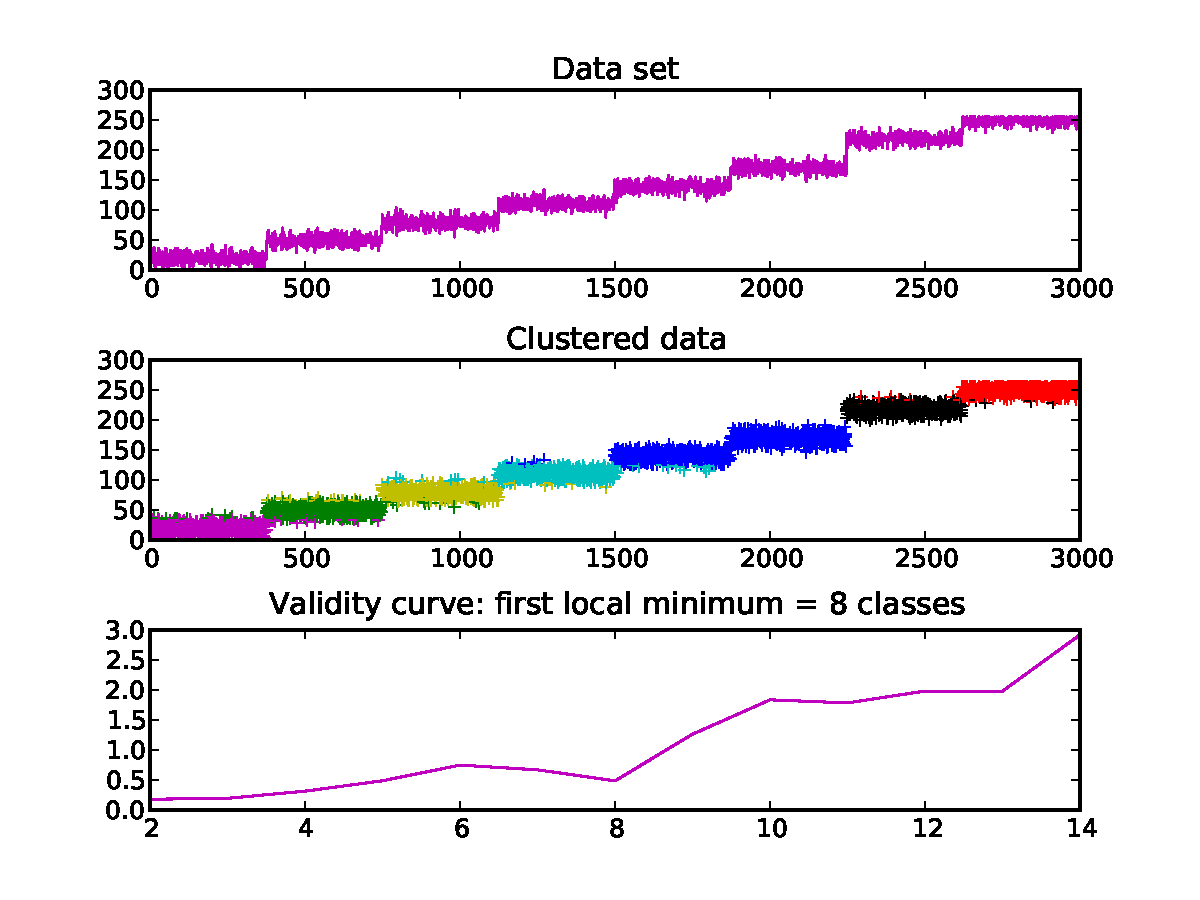
\includegraphics[trim= 10mm 10mm 10mm 10mm, clip, width=0.52\textwidth]{Evaluation/figure/me_3_3in1_1.pdf}}
			\subfloat[Classes rapprochées]{\label{fig:me_3_3in1}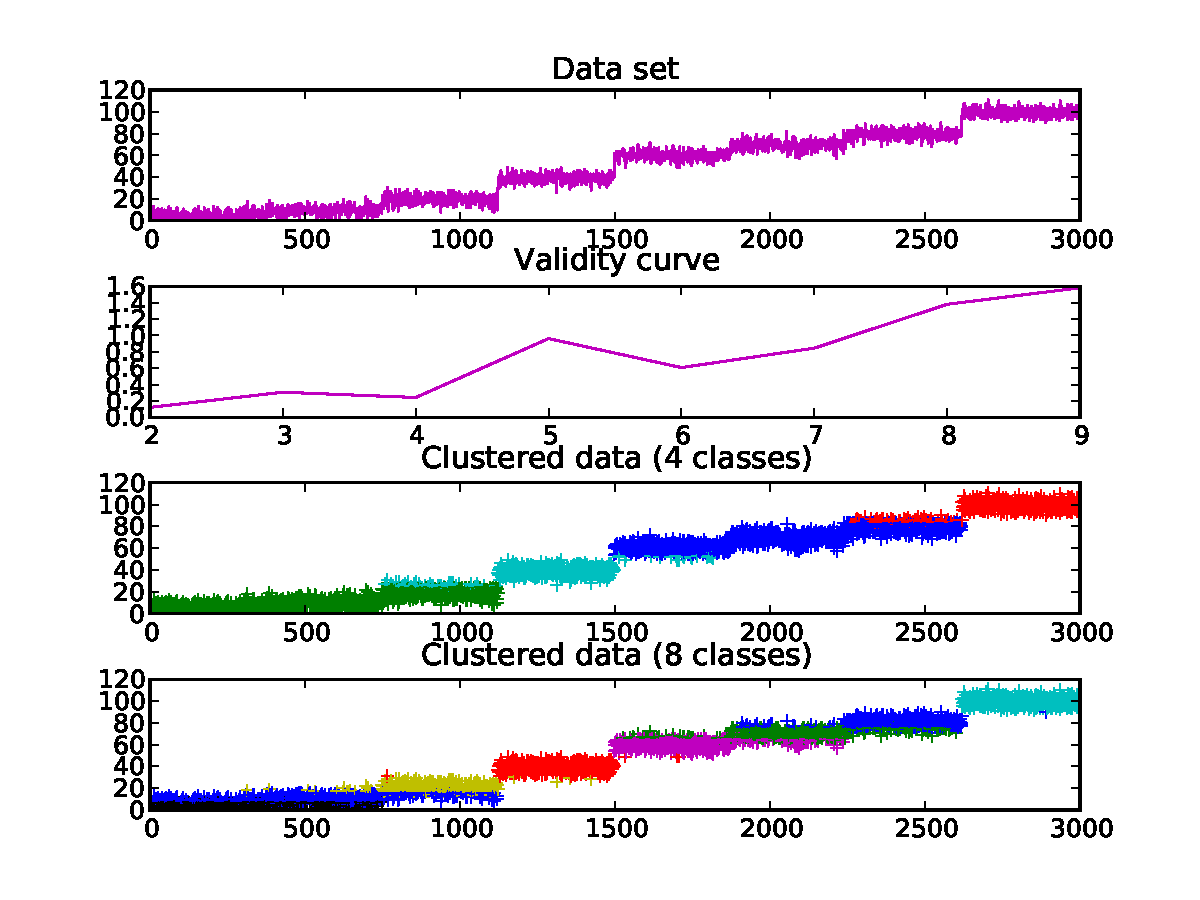
\includegraphics[trim= 10mm 10mm 10mm 10mm, clip, width=0.52\textwidth]{Evaluation/figure/me_3_3in1.pdf}}
			\caption{Mise en échec de l'algorithme de validation}
	\end{figure}
%	%%%%%%%%%%%%%%%%%%%%%%%%%%%%%%%%%%%%%%%%%%%%%%%%%%%
%	
	
	
	\subsection*{Temps de calcul: le coût d'une détermination automatique}
	Prenons l'exemple d'une image dont on ne connaît pas le nombre à priori de classe, on recherche entre 2 et $Nmax$ classes (ici $Nmax=14$). Il faudra environ 1 minute pour appliquer \emph{K-Means} de 2 à 14 classes et déterminer automatiquement qu'il y a 8 classes dans l'image. De part le moteur d'inférences, nous disposons directement du nombre de classes a priori, permettant ainsi d'éviter de faire des calculs inutiles ce qui s'avèrent être non négligeable dans cet exemple, puisque l'application direct de \emph{K-Means} à 8 classes ne prend que 5 secondes. La détermination automatique est, dans ce cas, est \textbf{12 fois plus lente}. Cela semble évident puisque qu'il y a douze cas à tester.

	
%	%%%%%%%%%%%%%%%%%%%%%%%%%%%%%%%%%%%%%%%%%%%%%%%%%%%
%	\begin{figure}[!ht]	%trim=l b r t  width=0.5\textwidth, 
%	  	\centering
%	  		\subfloat[Courbe de validité entre 2 et 14 classes]{\label{fig:me_3_0_no_interval}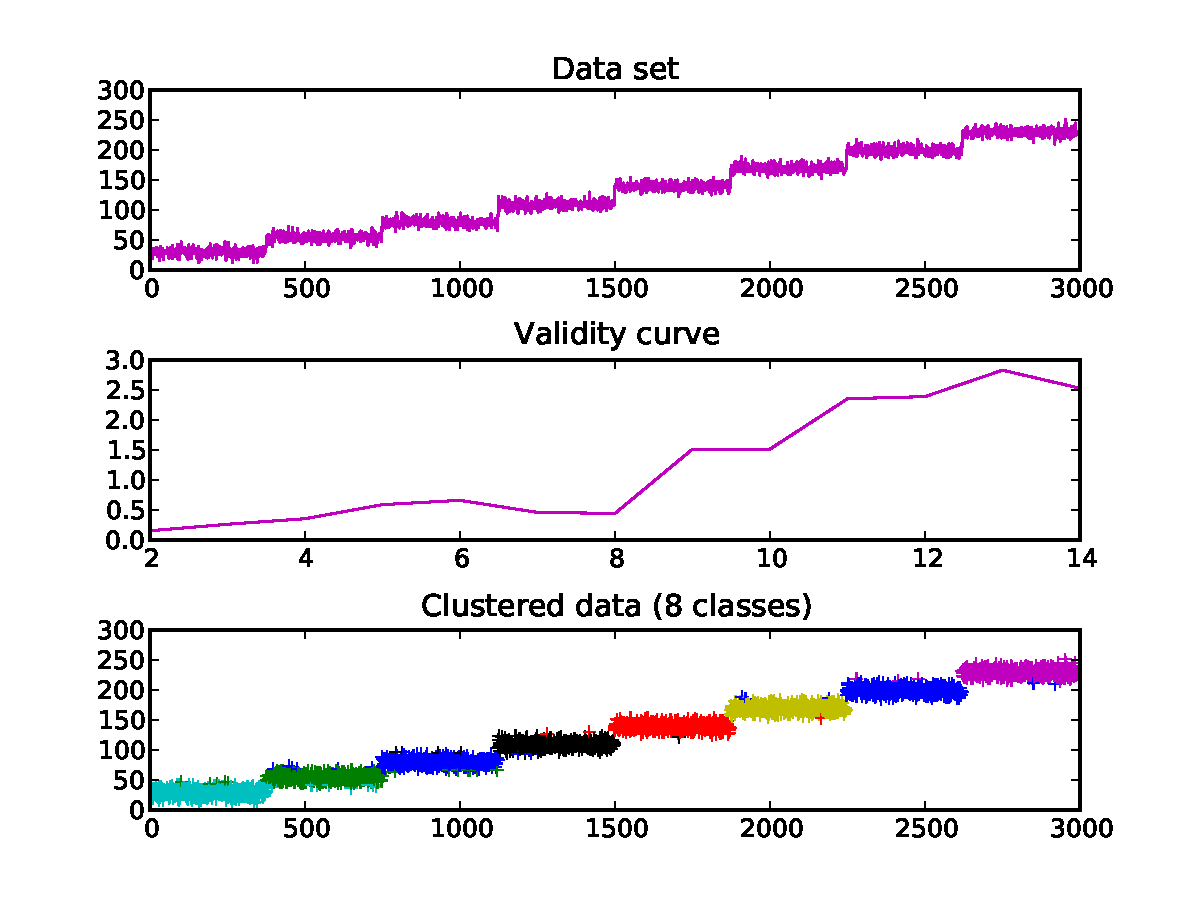
\includegraphics[trim= 10mm 55mm 10mm 9mm, clip, width=0.52\textwidth]{Evaluation/figure/me_3_0_no_interval.pdf}}
%			\subfloat[Courbe de validité entre 5 et 9 classes]{\label{fig:me_3_0_interval}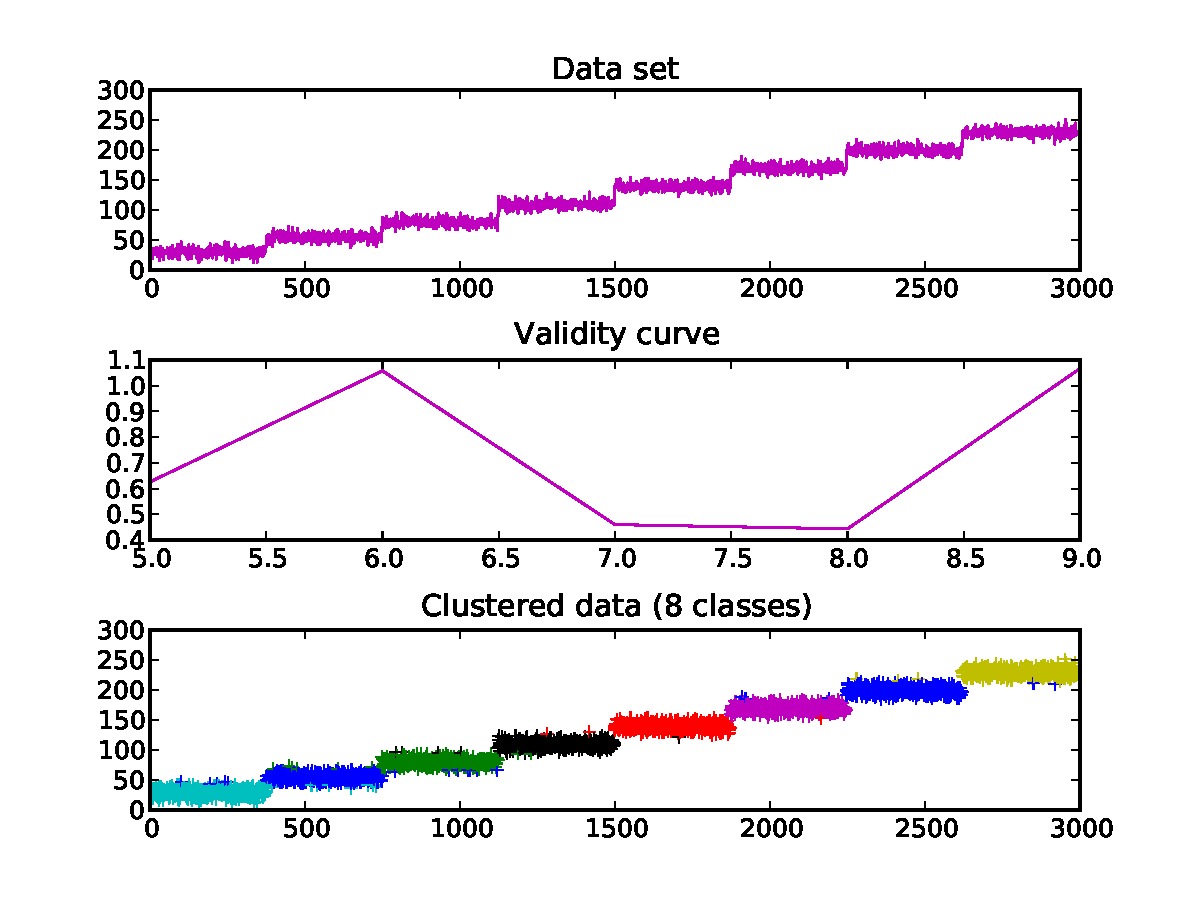
\includegraphics[trim= 10mm 55mm 10mm 9mm, clip, width=0.52\textwidth]{Evaluation/figure/me_3_0_interval.pdf}}
%			\caption{Variation de l'intervalle de recherche}
%	\end{figure}
%	%%%%%%%%%%%%%%%%%%%%%%%%%%%%%%%%%%%%%%%%%%%%%%%%%%%

	%%%%%%%%%%%%%%%%%%%%%%%%%%%%%%%%%%%%%%%%%%%%%%%%%%%%%%%%%%%%%%%%%%%%%%%%%%%%%%%%%%%%%%%%%%%%%%%%%%%%%%%%%%%%%%%%%%%%%
	%											INITIALISATION DES BARYCENTRES											%
	%%%%%%%%%%%%%%%%%%%%%%%%%%%%%%%%%%%%%%%%%%%%%%%%%%%%%%%%%%%%%%%%%%%%%%%%%%%%%%%%%%%%%%%%%%%%%%%%%%%%%%%%%%%%%%%%%%%%%
		\section{Relations photométriques et initialisation des centroïdes}
		Nous pouvons déterminer à partir des informations photométriques la position relative des classes dans l'histogramme (e.g. plus claire à droite, plus foncé à gauche). Cette information est particulièrement intéressante si l'on cherche une ou plusieurs classes qui sont entre deux autres segmentées (dont on connaît les centroïde) ou entre une segmentée et un extremum d'intensité. Malgré que cet aspect soit très dépendant du contexte, il est néanmoins non négligeable dans certains cas limites comme celui illustré ci-après. % et qu'il introduit des notions quantitatives

	La connaissance à priori du centroïde (proche de la notion de moyenne) de chaque classe de point est un paramètre que peut intégrer l'algorithme \emph{K-Means}, nous allons donc quantifier son apport. Prenons l'exemple d'une image à cinq classes (fig.~\ref{fig:me_4_img_1}) dont ont suppose que les classes A et D ont été segmentées et masquées (centroïdes de 25 et 150 en vert fig.~\ref{fig:me_4_hist_4}). On peut estimer une répartition à priori des centroïdes des classes B, C et E sachant que deux d'entre elles ont une intensité moyenne comprises entre celle de A et D, qu'une troisième est plus grande que D et que les intensités de l'image sont comprises entre 0 et 255 (image 8 bits). Dans cet exemple, l'estimation initiale des centroïdes relatifs à B et C sont répartis de manière équilibrée entre les intensités moyennes mesurées des classes A et E. L'estimation initiale du centroïde relatif à E correspond à l'intensité moyenne entre celle de D et l'intensité maximale de l'image (voir les positions des centroïdes en vert sur la fig.~\ref{fig:me_4_hist_4}). %Voir éq.~\ref{eq:mean_estimations} et hist.~\ref{fig:me_4_hist_4}.


	%%%%%%%%%%%%%%%%%%%%%%%%%%%%%%%%%%%%%%%%%%%%%%%%%%%
	\begin{figure}[!ht]	%trim=l b r t  width=0.5\textwidth, 
	  	\centering
	  		\subfloat[Image initiale]{\label{fig:me_4_img_1}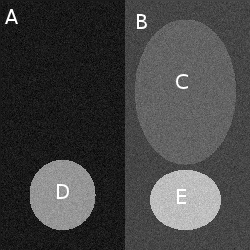
\includegraphics[trim= 0mm 0mm 0mm 0mm, clip, height=0.23\textwidth]{Evaluation/figure/me_4_img_1.png}}	\hspace{2em}
			\subfloat[Image masquée]{\label{fig:me_4_img_2}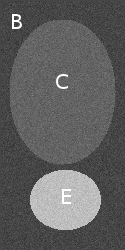
\includegraphics[trim= -20mm 0mm -10mm 0mm, clip, height=0.23	\textwidth]{Evaluation/figure/me_4_img_2.png}}	\hspace{2em}
			\subfloat[Estimation des moyennes]{\label{fig:me_4_hist_4}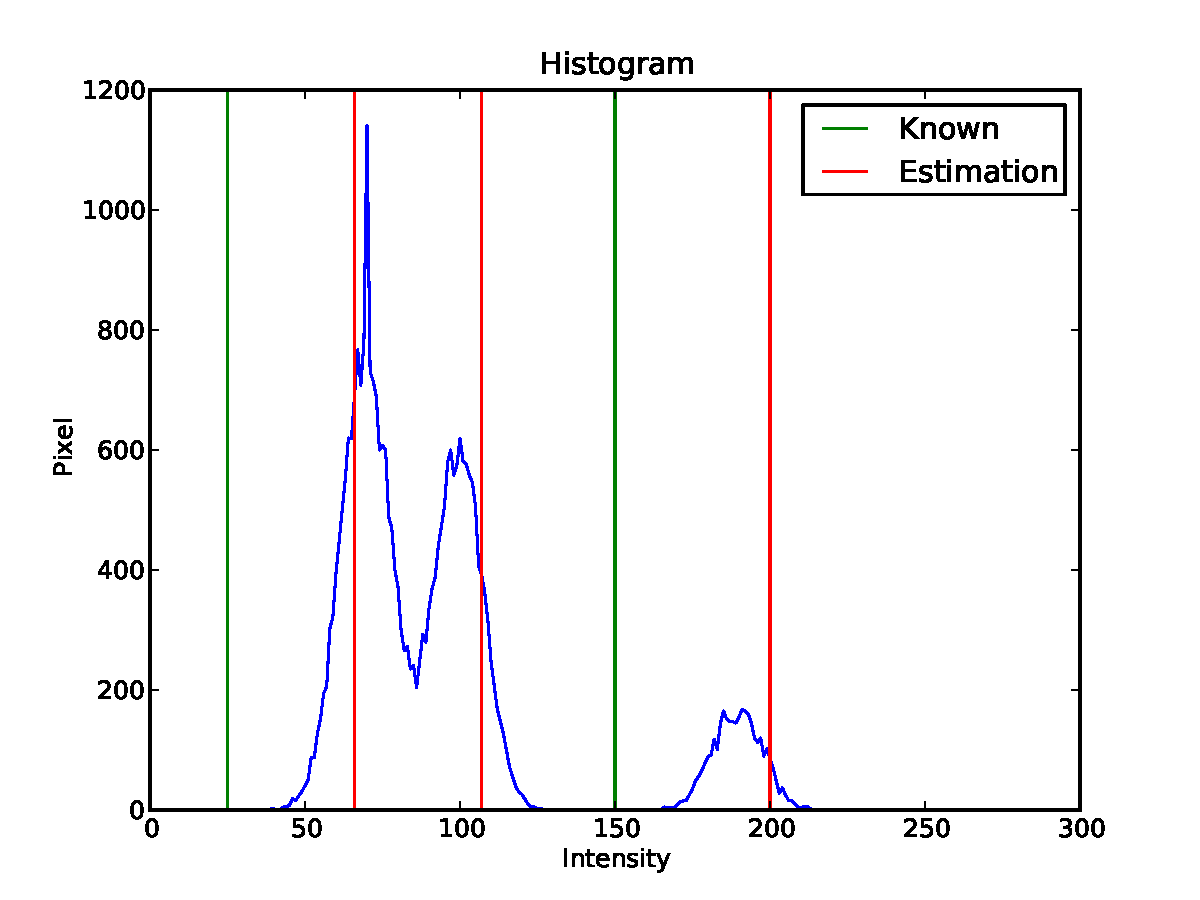
\includegraphics[trim= 5mm 5mm 5mm 15mm, clip, width=0.33\textwidth]{Evaluation/figure/me_4_hist_4.pdf}}
			%\subfloat[Variance proche de 33000]{\label{fig:me_4_point}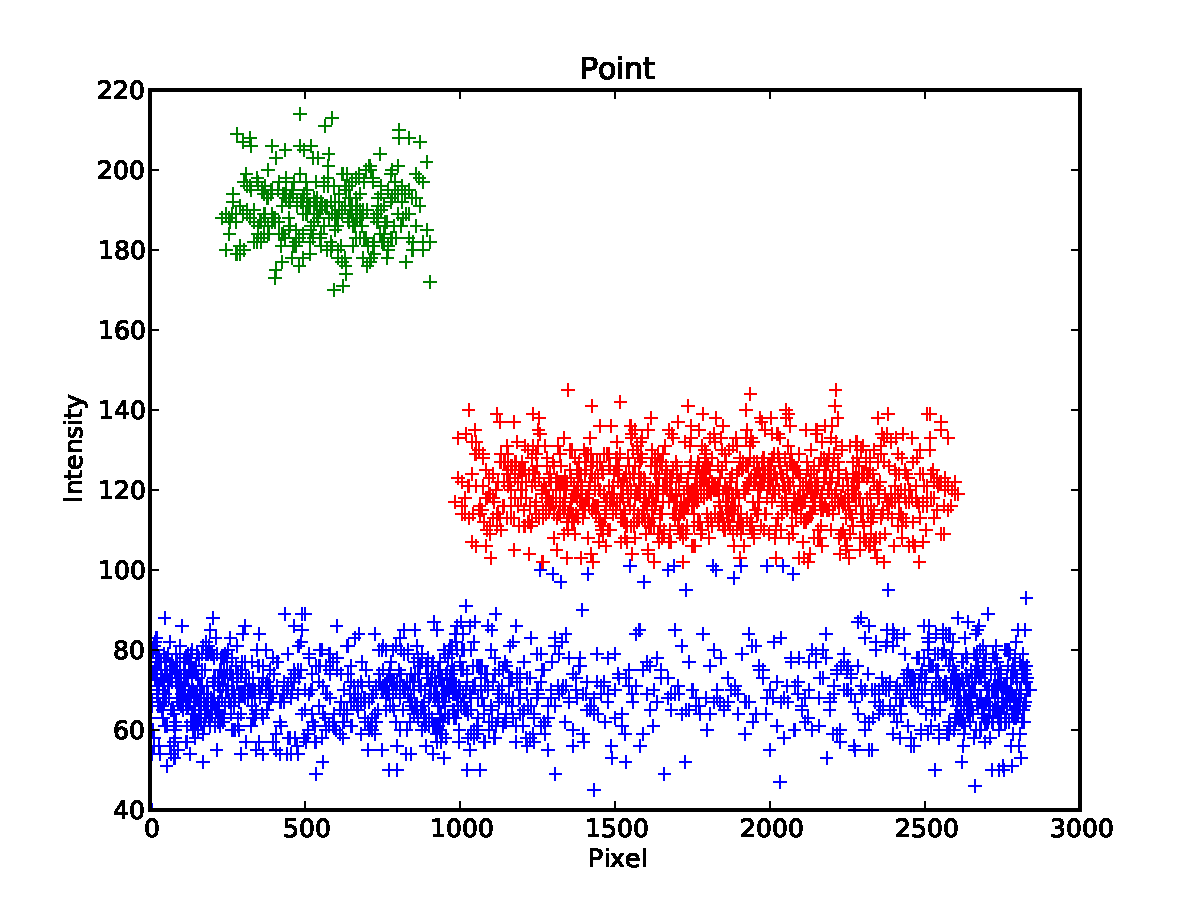
\includegraphics[trim= 5mm 5mm 5mm 5mm, clip, width=0.38\textwidth]{Evaluation/figure/me_4_point.pdf}}
		  	\caption{Images et histogrammes associés}
	\end{figure}
	%%%%%%%%%%%%%%%%%%%%%%%%%%%%%%%%%%%%%%%%%%%%%%%%%%%

		Le tableau suivant montre les résultats obtenus avec \emph{K-Means} initialisé avec des moyennes aléatoires puis calculés à partir des connaissances à priori dans le cas où la ROI correspond aux régions B, C et E (fig.~\ref{fig:me_4_img_2}) :
		
	\begin{center}
		\begin{tabular}{|l|c|c|c|c|c|c|c|c|}
			\hline
			 \textbf{$\sum$ variances} & \textbf{1}	& \textbf{2} & \textbf{3}	& \textbf{4} & \textbf{5}	& \textbf{6}  & \textbf{8}	& \textbf{9} \\
			\hline
				Aléatoire	 			& 168131	& 168009	& 743240		& 168405	& 168131		& 168118	& 743240		& 743174	\\
			 	Prédéfinie				& 168131	& 168131	& 168131		& 168131	& 168131		& 168131 	& 168131		& 168131	\\
			 \hline	
		\end{tabular}
		\captionof{table}{Sommes des variances}
		\label{tab:centroid_benefit}
	\end{center}
	
		La somme des variances (inerties) témoigne de la dispersion des valeurs par rapport à la moyenne, on constate qu'elle est stationnaire pour une initialisation avec des moyennes prédéfinies alors qu'elle fluctue dans le cas de l'initialisation aléatoires. Les valeurs sont très dépendantes du contexte mais la fluctuation pourrait être vérifiée dans d'autre cas. Les figures ci-après montrent quelques résultats de classification pour trois différentes inerties. Elles illustrent la relation entre une inertie élevée et la répartition des points entre les classes.	%Les trois premières figures ci-dessous montrent la variabilité de la segmentation dans le cas des initialisations aléatoires, les trois suivantes la stabilité lors d'initialisations prédéfinies :
		 %les intervalles trouvés sont identiques et que le nombre d'itérations ne varie pas pour les moyennes prédéfinies. La grandeur la plus intéressante est la variance (inertie) car elle informe sur la dispersion des valeurs par rapport à la moyenne et donc plus elle est faible, plus les classes sont compactes. 
				
	%%%%%%%%%%%%%%%%%%%%%%%%%%%%%%%%%%%%%%%%%%%%%%%%%%%
	\begin{figure}[!ht]	%trim=l b r t  width=0.5\textwidth, 
	  	\centering
			\subfloat[Variance de 168131]{\label{fig:me_4_point_0}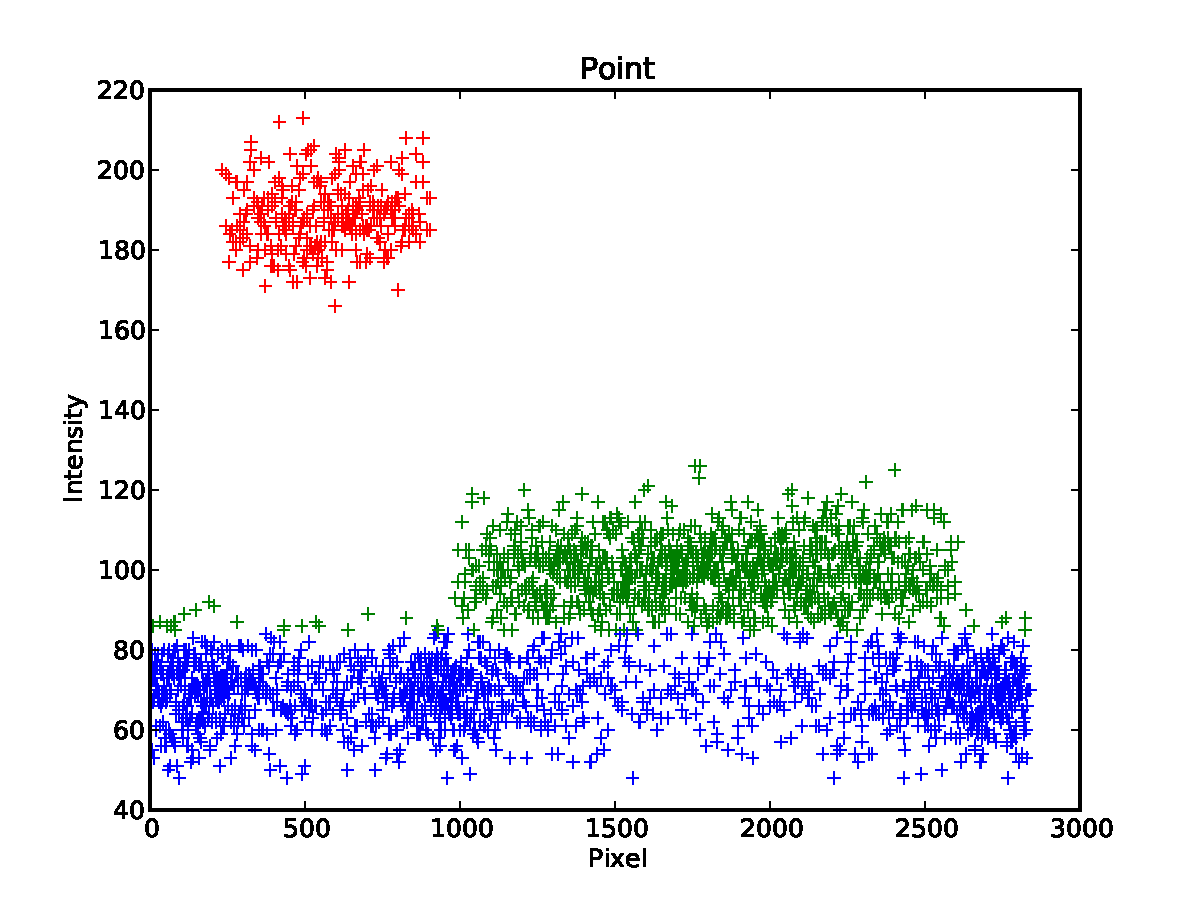
\includegraphics[trim= 5mm 5mm 5mm 5mm, clip, width=0.35\textwidth]{Evaluation/figure/me_4_point_random_1_168131.pdf}}
			\subfloat[Variance de 168405]{\label{fig:me_4_point_2}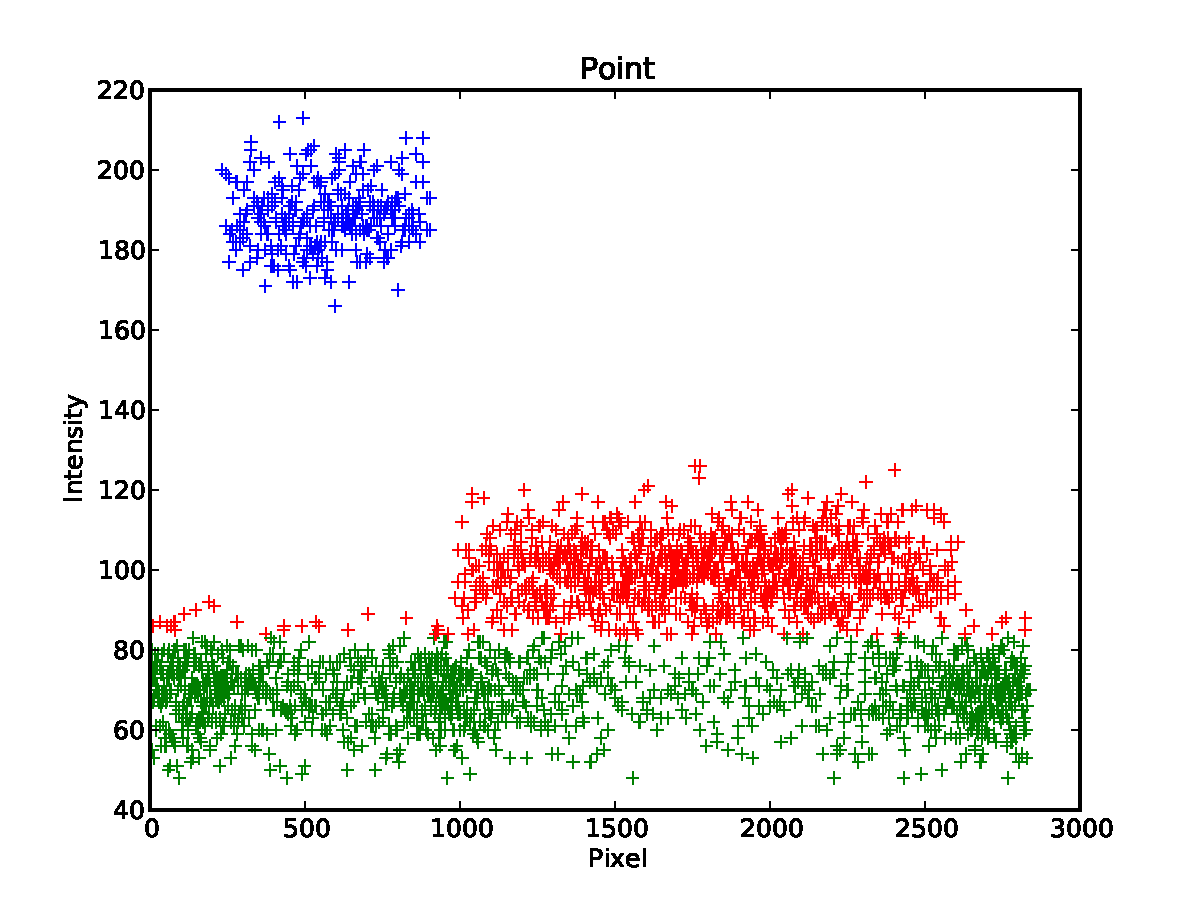
\includegraphics[trim= 5mm 5mm 5mm 5mm, clip, width=0.35\textwidth]{Evaluation/figure/me_4_point_random_4_168405.pdf}}
			\subfloat[Variance de 743240]{\label{fig:me_4_point_1}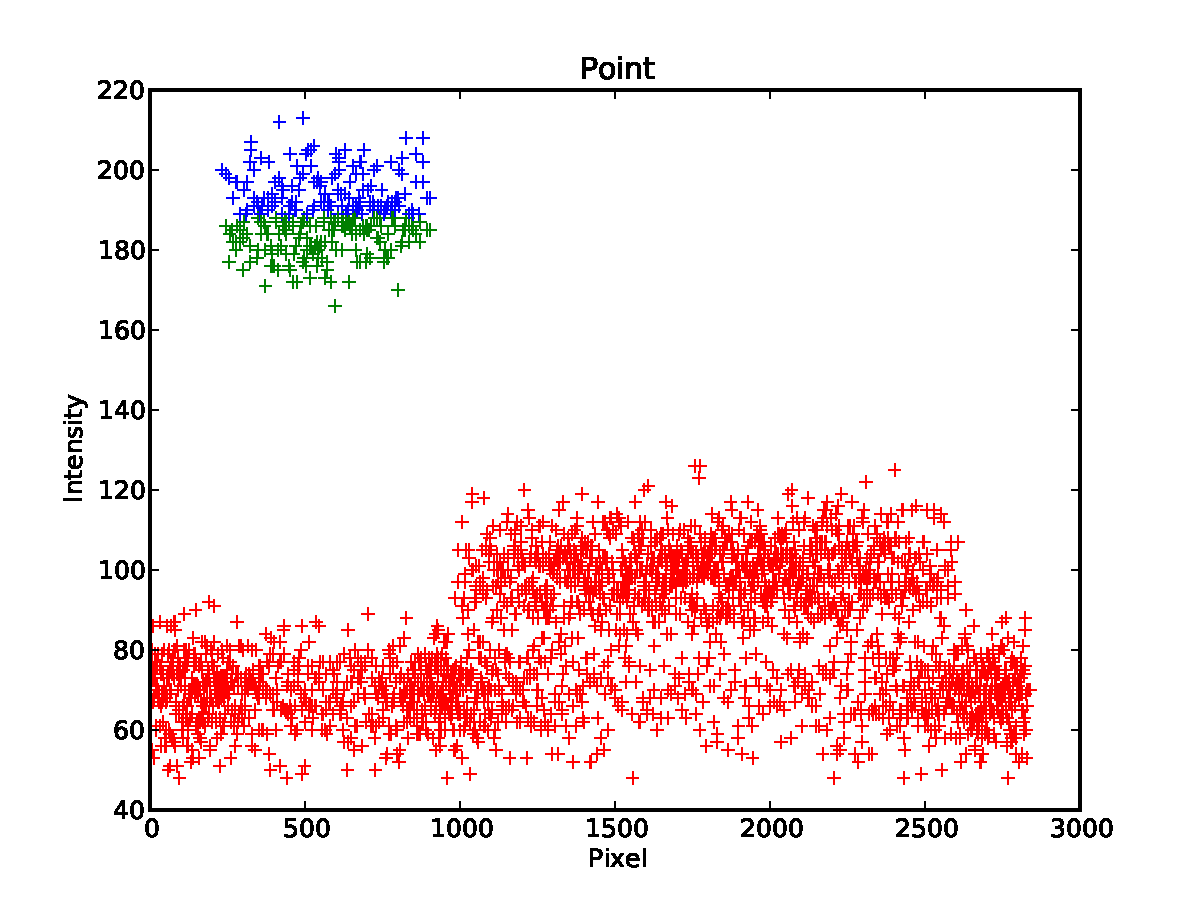
\includegraphics[trim= 5mm 5mm 5mm 5mm, clip, width=0.35\textwidth]{Evaluation/figure/me_4_point_random_3_743240.pdf}}	\\		
			%\subfloat[Variance de 168131]{\label{fig:me_4_point_0}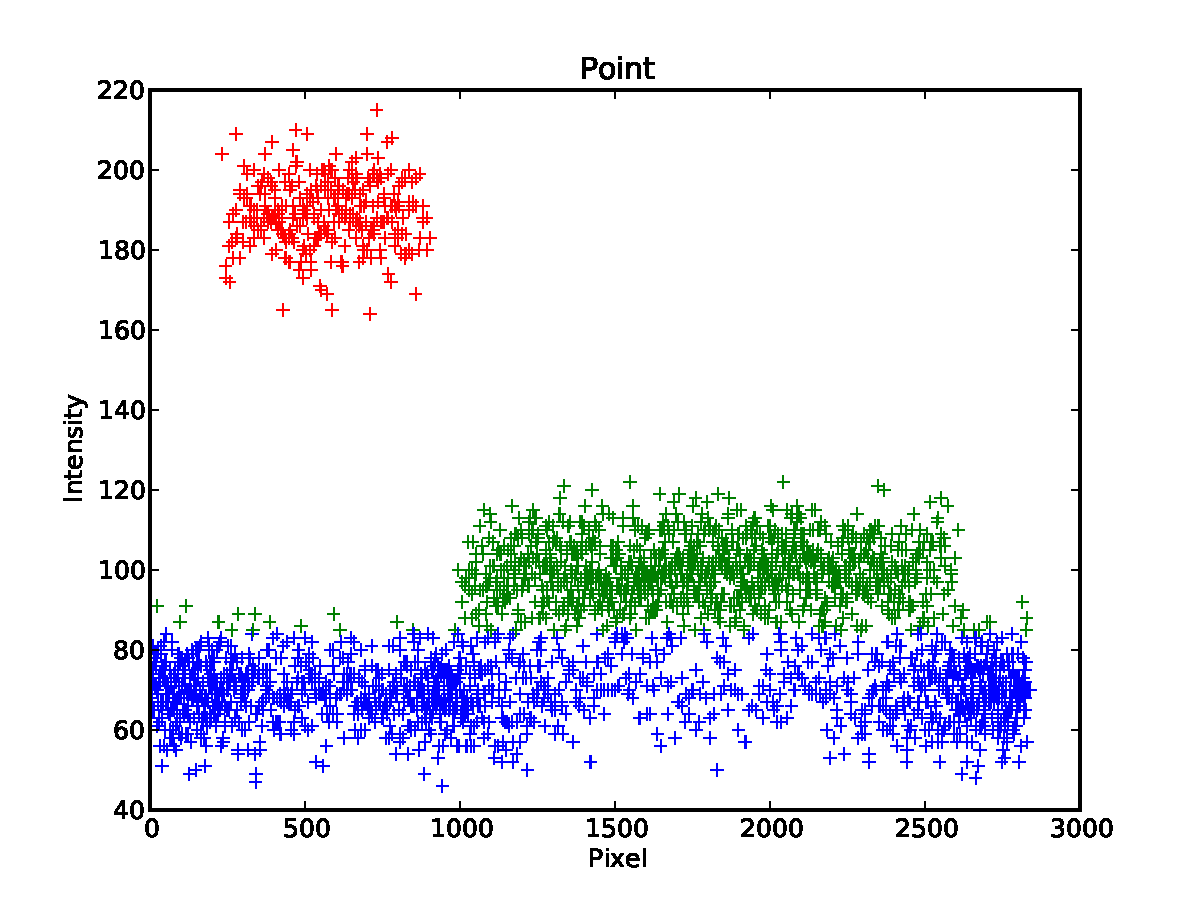
\includegraphics[trim= 5mm 5mm 5mm 5mm, clip, width=0.35\textwidth]{Evaluation/figure/me_4_point_manual_0.pdf}}
			%\subfloat[Variance de 168131]{\label{fig:me_4_point_1}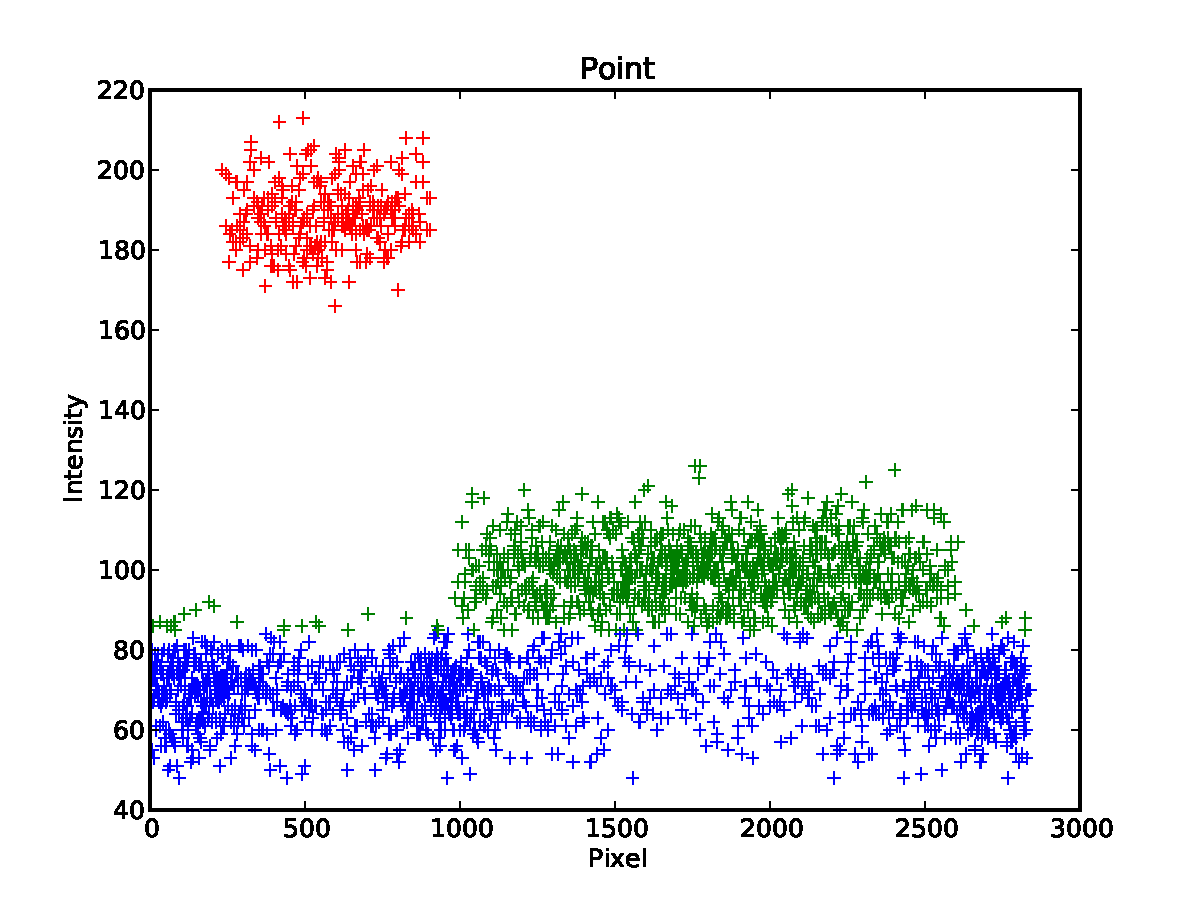
\includegraphics[trim= 5mm 5mm 5mm 5mm, clip, width=0.35\textwidth]{Evaluation/figure/me_4_point_manual_1_168131.pdf}}
			%\subfloat[Variance de 168131]{\label{fig:me_4_point_2}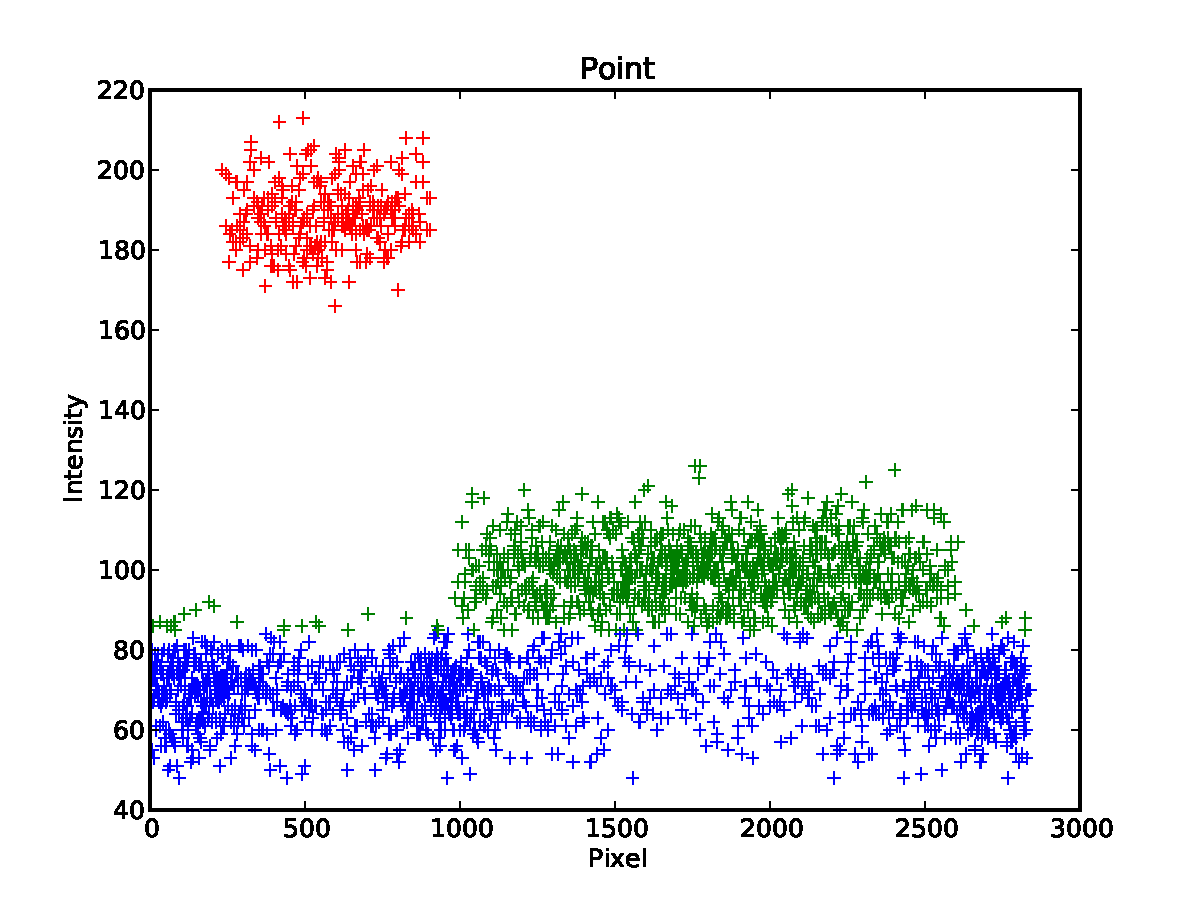
\includegraphics[trim= 5mm 5mm 5mm 5mm, clip, width=0.35\textwidth]{Evaluation/figure/me_4_point_manual_3_168131.pdf}}
		  	\caption{Partitionnement et inertie : la figure (c) montre une classification inacceptable.}
	\end{figure}
	%%%%%%%%%%%%%%%%%%%%%%%%%%%%%%%%%%%%%%%%%%%%%%%%%%%



		%{\bf Arguments: initialisation = valeurs relatifs = problème quantitatif hors graphe non quantitatif. Mais déjà info de position relative (E est à droite de D) et (B,C) entre A et D: exploitable. bénéfice vraiment fonction du contexte mais non négligeable dans certains cas limites, comme celui illustré ici.}
		
		

	%%%%%%%%%%%%%%%%%%%%%%%%%%%%%%%%%%%%%%%%%%%%%%%%%%%
	%\begin{equation}
	%	 \begin{split}
	  		%L_t(1) = & \left\{ i \in \left( G_T^{\infty}(G_{T,t}^{-1}(1)) \cap ( S \setminus S_t ) \right) \;|\; \left( G_{T,t}^{-1} (i) \cap G_{T,t}^{-1} (1) \neq \emptyset \right) \right\} \cup  G_{T,t}^{-1}(1)\\
		 			%= & \left\{ i \in \left( \{1,2,3,4,6,5\} \cap \{1,3,4,6,5\} \right) \;|\; \left( G_{T,t}^{-1} (i) \cap \{0\} \neq \emptyset \right) \right\} \cup  \{0\}\\
		 			%= & \left\{1 \right\} \cup  \{0\}\\
	%	\bar{B} = & \bar{A} + (\bar{D}-\bar{A}/(2+1)) =  25 + (150-25)/3 =  66.67 		\\
	%	\bar{C} = & \bar{D} - (\bar{D}-\bar{A}/(2+1)) = 150 - (150-25)/3 = 108.34 		\\
	%	\bar{E} = & \bar{D} + (MaxI - \bar{D} /(1+1)) = 150 + (255 - 150) / 2 = 202.5	\\	 			
	 %\end{split}
		%\label{eq:mean_estimations}
	%\end{equation}
	%%%%%%%%%%%%%%%%%%%%%%%%%%%%%%%%%%%%%%%%%%%%%%%%%%%
		
		
		

	%%%%%%%%%%%%%%%%%%%%%%%%%%%%%%%%%%%%%%%%%%%%%%%%%%%%%%%%%%%%%%%%%%%%%%%%%%%%%%%%%%%%%%%%%%%%%%%%%%%%%%%%%%%%%%%%%%%%%
	%													IMAGE SYNTHETIQUE												%
	%%%%%%%%%%%%%%%%%%%%%%%%%%%%%%%%%%%%%%%%%%%%%%%%%%%%%%%%%%%%%%%%%%%%%%%%%%%%%%%%%%%%%%%%%%%%%%%%%%%%%%%%%%%%%%%%%%%%%

%	\section{TO REMOVE Images synthétiques}
%		\subsection{Vérité terrain}
%		Appliquons le mode opératoire à une images synthétiques~\ref{fig:img_syn} pour laquelle on a générer les masques correspondants au trois structures. On pourra assimiler ces structures au foie, à une tumeur et au vaisseaux interne au foie. La disposition spatiale des structures n'influence pas notre démarche de caractérisation puisque l'on travaille uniquement sur la photométrie ici.
%		Notons, pour comparaison, les valeurs utilisées pour générer l'image : trois structures d'intensité 75, 115 et 160 sur une échelle 0 à 255 de niveaux de gris, bruité avec un bruit gaussien d'écart type 4.


%	%%%%%%%%%%%%%%%%%%%%%%%%%%%%%%%%%%%%%%%%%%%%%%%%%%%
%	\begin{figure}[!ht]	%trim=l b r t  width=0.5\textwidth, 
%	  \centering
%			\subfloat[Image synthétique]{\label{fig:img_syn}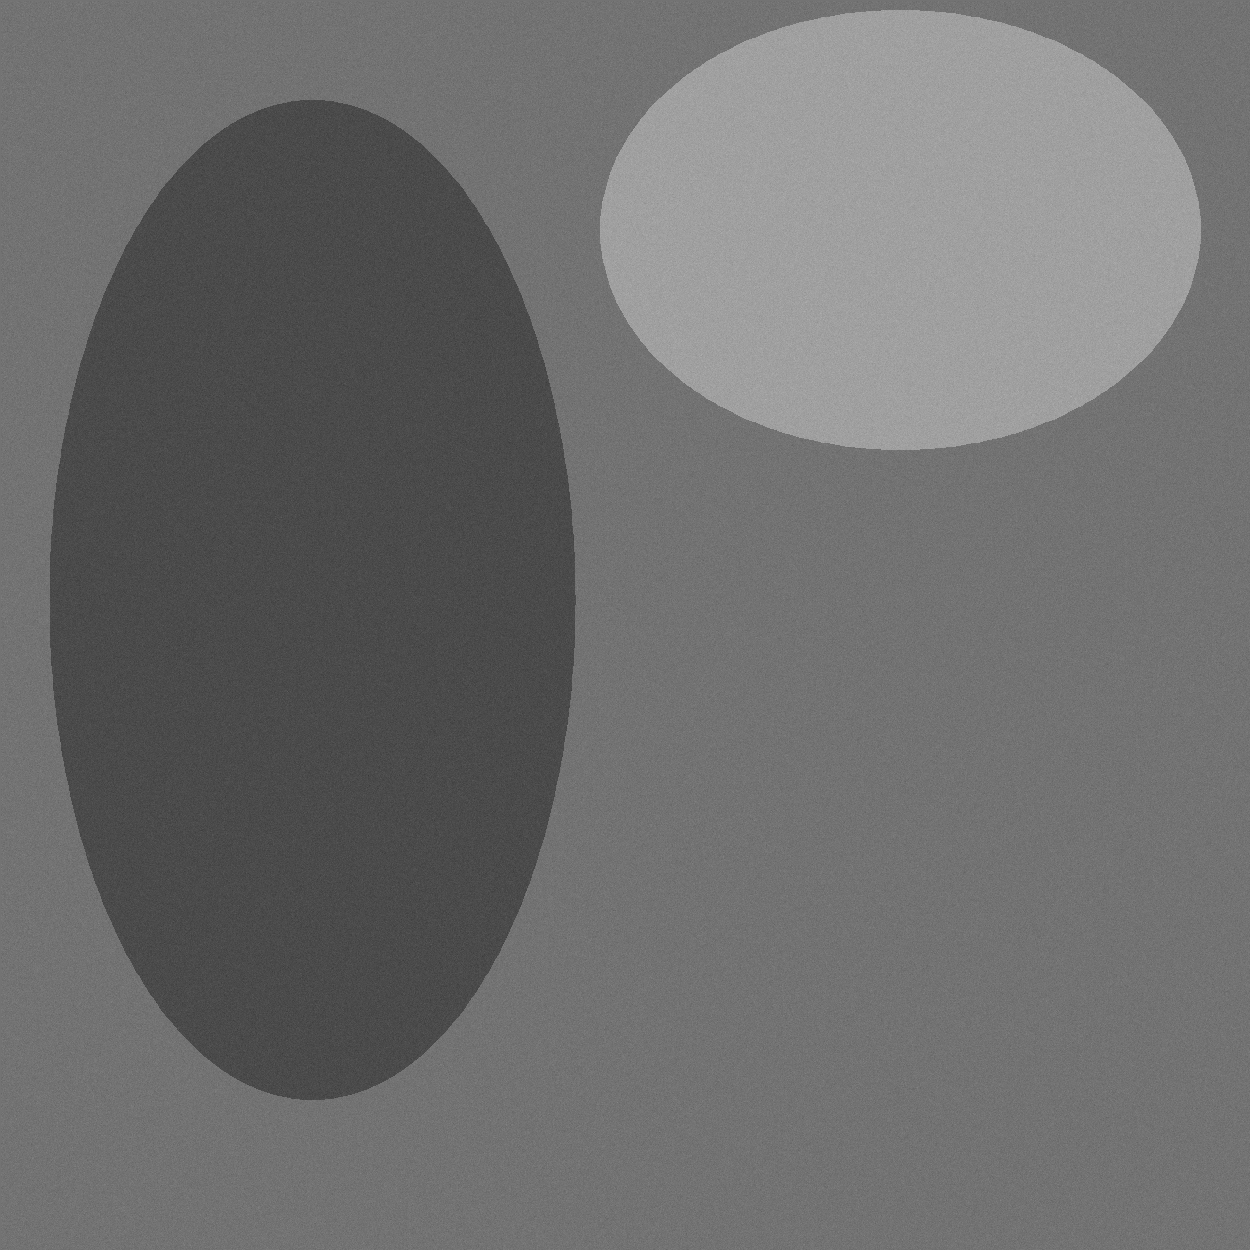
\includegraphics[trim= 0mm 0mm 0mm 0mm, clip, width=0.2\textwidth]{Evaluation/figure/img_syn.png}}\hspace{2em}
%		  	\subfloat[Masque du foie]{\label{fig:mask_syn_liver}\fbox{
\includegraphics[trim= 0mm 0mm 0mm 0mm, clip, width=0.2\textwidth]{Evaluation/figure/mask_syn_liver.png}}}\hspace{1em}
%		   	\subfloat[Masque tumeur]{\label{fig:mask_syn_tumor}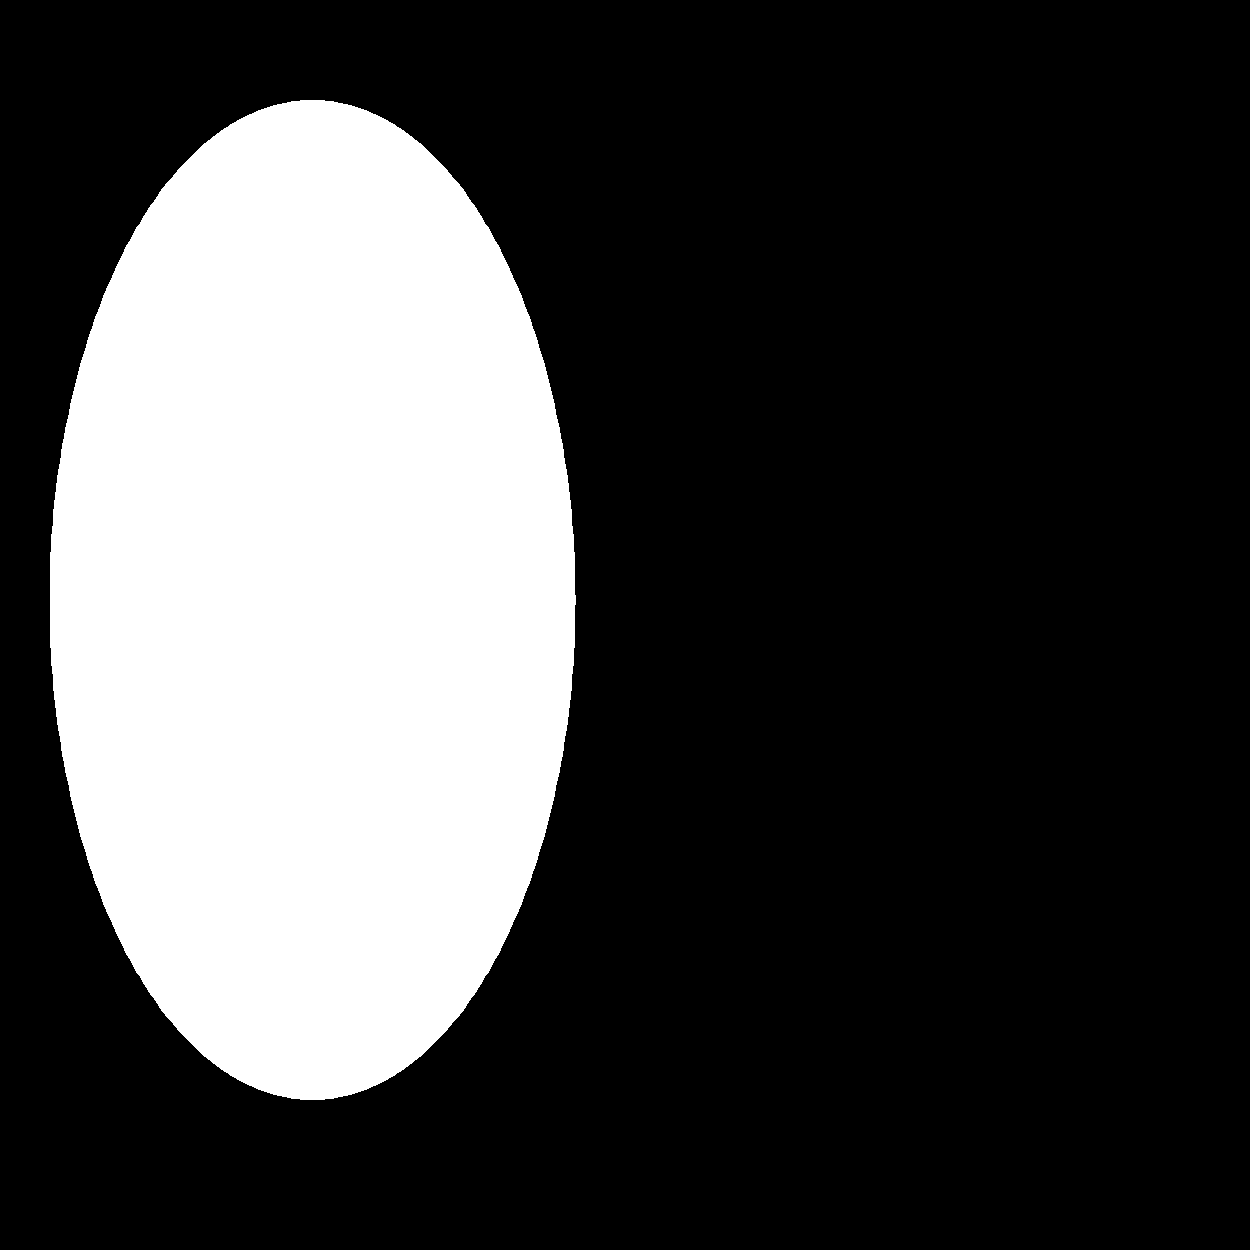
\includegraphics[trim= 0mm 0mm 0mm 0mm, clip, width=0.2\textwidth]{Evaluation/figure/mask_syn_tumor.png}}\hspace{1em}
%		  	\subfloat[Masque vaisseaux]{\label{fig:mask_syn_vessel}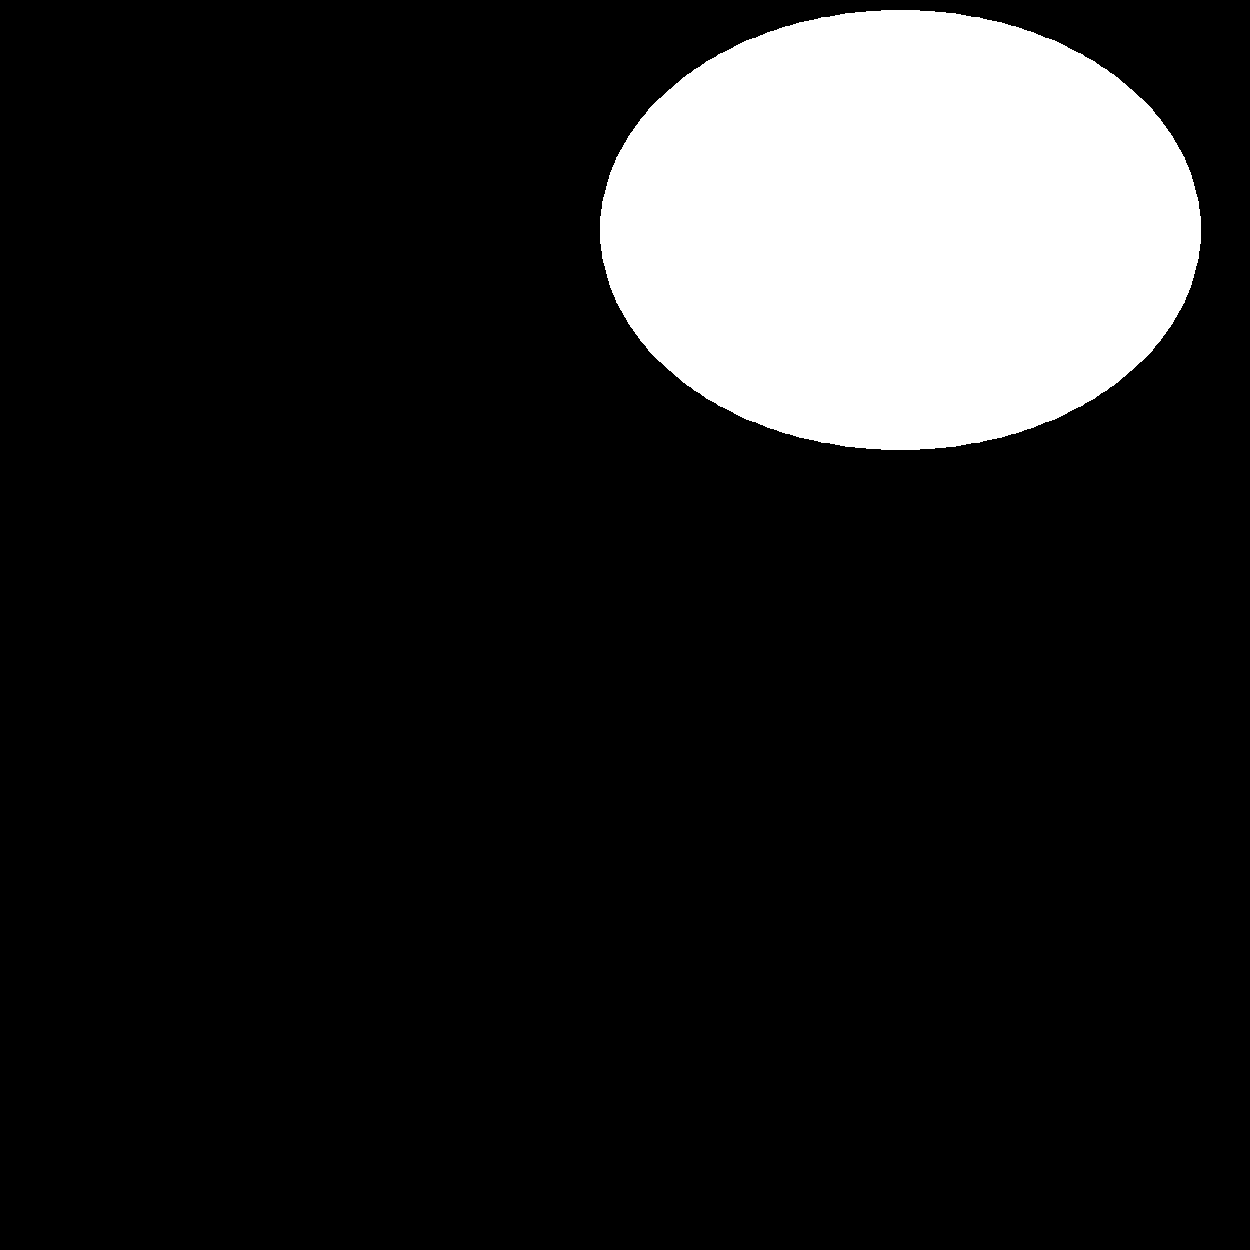
\includegraphics[trim= 0mm 0mm 0mm 0mm, clip, width=0.2\textwidth]{Evaluation/figure/mask_syn_vessel.png}}		  
%		\caption{Ensemble des données synthétiques}		  
%	\end{figure}
%	%%%%%%%%%%%%%%%%%%%%%%%%%%%%%%%%%%%%%%%%%%%%%%%%%%%


%	%%%%%%%%%%%%%%%%%%%%%%%%%%%%%%%%%%%%%%%%%%%%%%%%%%%
%		\begin{figure}[!ht]	%trim=l b r t  width=0.5\textwidth, 
%		  \centering
%				\fbox{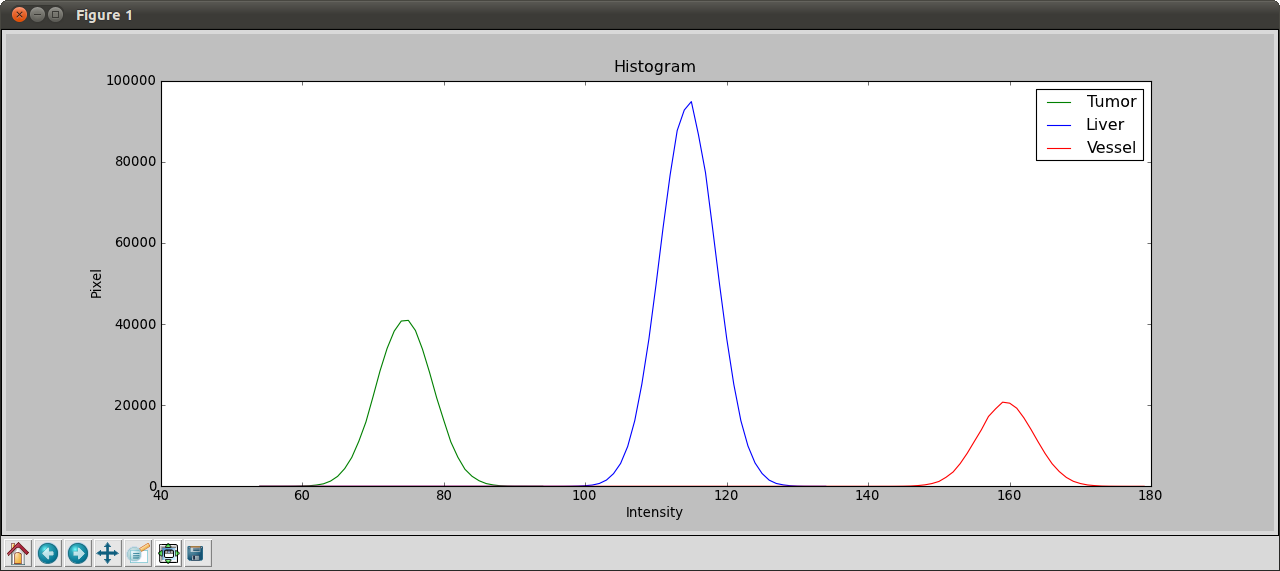
\includegraphics[trim= 30mm 15mm 40mm 20mm, clip, width=0.7\textwidth]{Evaluation/figure/3_histo_synthese.png}}
%			\caption{Histogrammes des distributions}		  
%			\label{fig:3_histo_synthese}
%		\end{figure}
%	%%%%%%%%%%%%%%%%%%%%%%%%%%%%%%%%%%%%%%%%%%%%%%%%%%%
%	
%	Le tableau ci-dessous contient les résultats des estimation des distributions~\ref{fig:3_histo_synthese} de chaque structure :

%	\begin{center}
%		\begin{tabular}{|l|lllll|}
%			\hline
%			%\textbf{Patient} & \multicolumn{2}{|c|}{\textbf{Tumeur [min,mu,max]}} & \multicolumn{2}{|c|}{\textbf{Foie [min,mu,max]}} & \multicolumn{2}{|c|}{\textbf{Système vénal [min,mu,]}} \\
%			%\hline
%			Nom						& Moyenne	& Médiane	& Écart type& Minimum 	& Maximum	\\
%			\hline
%				Tumeur				& 74.5 		& 74.0 		& 4.0 		& 54 		& 94		\\
%			 	Foie				& 114.5 	& 115.0 	& 4.0 		& 97 		& 134 		\\
%			 	réseau vasculaire		& 159.5 	& 159.0		& 4.0 		& 142 		& 179 		\\
%			 \hline	
%		\end{tabular}
%		\captionof{table}{Résultats des estimations}
%		\label{tab:estimation_references_synthese}
%	\end{center}
%	
%	%On retrouve bien les valeurs moyennes et écart-types identiques (arrondi à la valeur entière) à celle utilisées lors de la génération de l'image.

%		\subsection{Estimation}
%		Tentons maintenant d'identifier la tumeur au sein de l'image en appliquant l'algorithmes de segmentation \emph{K-Means}. Nous évaluerons les résultats par rapport à la vérité terrain. On montrera l'intérêt de la connaissance du nombre de classes à priori ainsi que des masques.
%		
%		Tout d'abord considérons l'image dans sont ensemble (sans masque ni connaissance sur le nombre de classes) :


%	\begin{center}
%		\begin{tabular}{|l|llllllllll|l|l|}
%			\hline
%			 & \multicolumn{2}{|c|}{Classe 1} & \multicolumn{2}{|c|}{Classe 2} & \multicolumn{2}{|c|}{Classe 3} & \multicolumn{2}{|c|}{Classe 4} & \multicolumn{2}{|c|}{Classe 5} & Ité. & Valide\\
%			\hline
%			Nb classes & Min	& Max 	& Min	& Max & Min	& Max	& Min	& Max & Min	& Max & &	\\
%			\hline
%			2	& 54 & 108 & 109 & 179												& & & & & &		& 3		&  	0\\
%			3	& 54 & 108 & 109 & 134 & 142 & 179	 									& & & &		& 3 	&  	1\\
%%			4	& 2 & 44 & 45 & 95 & 96 & 135 & 136 & 208 									& &		& 7  	& 	3\\
%%			5	& 2 & 43 & 44 & 89 & 90 & 113 & 114 & 140 & 141 & 208								& 5		&	1\\
%			\hline
%		\end{tabular}
%		\captionof{table}{Résultats des estimations}
%		\label{tab:kmean_full_img_syn}
%	\end{center}

%		Maintenant on applique le masque correspondant à la tumeur :
%		
%		
%		Si l'on connaît le nombre de classes, on retrouve parfaitement la vérité terrain d'ou l'intérêt de la connaissance à priori.



